\documentclass[letterpaper,12pt]{book}

% TODO: since this is a submission to US-based NIST, we use a "letter"
% paper size. However, it is tempting to use A4 to teach them the glory
% of the metric system.

% !TeX root = ../falcon.tex

% This file contains the packages
\usepackage[T1]{fontenc}
\usepackage[utf8x]{inputenc}
\usepackage[english]{babel}
\usepackage{lmodern}
\usepackage{fullpage}
\usepackage{graphicx}
\usepackage{url}
\usepackage[dvipsnames]{xcolor}     % For colors
% @author Thomas Prest
% @author Pierre-Alain Fouque
% @author Jeffrey Hoffstein
% @author Paul Kirchner
% @author Vadim Lyubashevsky
% @author Thomas Pornin
% @author Thomas Ricosset
% @author Gregor Seiler
% @author William Whyte
% @author Zhenfei Zhang
% @copyright The authors


\definecolor{coral}{RGB}{255,87,40}
\definecolor{cblue}{RGB}{31, 117, 254}
\definecolor{mantis}{RGB}{116, 195, 101}
\definecolor{shamrock}{RGB}{0, 158, 96}
\definecolor{emerald}{RGB}{80, 200, 120}
\definecolor{france}{RGB}{49, 140, 231}
\definecolor{gold}{RGB}{249,196,95}
\definecolor{klein}{RGB}{0,46,167}
\definecolor{ultramarine}{RGB}{63,0,255}
\definecolor{navy}{RGB}{0,0,128}
\definecolor{midnight}{RGB}{25,25,112}
\definecolor{burgundy}{RGB}{144, 0, 32}

%%%%%%%%%%%%%%%%%%%%%%%%%%%%%%%%%%%%%%%%%%%%%%%%%%%%%%%%%%%%
\colorlet{one}{gold}
\colorlet{two}{black!60!cblue}
% \colorlet{two}{midnight}
\colorlet{three}{gold!20}
\colorlet{four}{black!20!cblue!20}
\colorlet{five}{shamrock}


\colorlet{color_cite}{burgundy}
\colorlet{color_url}{navy}
\colorlet{color_link}{navy}

\usepackage[%
% pdftex = true,%
colorlinks,%
citecolor=color_cite,%
backref=page,%
linkcolor=color_link,%
linktocpage=true,%
% draft=false,%
urlcolor=color_url,%
% https://tex.stackexchange.com/a/26530/176500
pdfauthor={%
	Pierre-Alain Fouque, Jeffrey Hoffstein, Paul Kirchner, Vadim Lyubashevsky, Thomas Pornin, Thomas Prest, Thomas Ricosset, Gregor Seiler, William Whyte, Zhenfei Zhang%
},%
pdftitle={Falcon: Fast-Fourier Lattice-based Compact Signatures over NTRU},%
% https://tex.stackexchange.com/a/156404/176500
hypertexnames=false,
]{hyperref}
\usepackage{xspace}
\usepackage{tabularx}
\usepackage[bottom]{footmisc}
\usepackage{numprint}

%%%
%%% For algorithms
%%%
\usepackage[noend]{algpseudocode}
\usepackage{algorithm}
%\usepackage{algorithmicx}


%%%
%%% Tikz
%%%
\usepackage{tikz}
\usetikzlibrary{matrix,calc}
\usetikzlibrary{tikzmark}
\usetikzlibrary{decorations.pathreplacing}
\usetikzlibrary{arrows,shapes.geometric,arrows.meta}
\tikzset{
line/.style = {draw, -latex'}
}

%%%
%%% These packages will probably be useful
%%%
\usepackage{pifont}
\usepackage{scrextend}
\usepackage{multirow}   % To fuse rows in tables
\usepackage{hhline}     % For double lines in tables
\usepackage{amsmath}    % AMS Math symbols
\usepackage{amssymb}    % AMS symbols
\usepackage{stmaryrd}   % Math stuff
\usepackage{array}      % for "\newcolumntype" macro
\usepackage{enumitem}   % For fancy enumerate and itemize
\usepackage{mathtools}
\usepackage{multicol}
\usepackage{cleveref}
\usepackage{etoolbox}   % Macro generation
\usepackage{titlesec}   % Change space before/after titles
\usepackage[textwidth=40mm]{todonotes}
\usepackage[nomessages]{fp}% http://ctan.org/pkg/fp

% Font choices:
%   eb-garamond with matching math mode and "modern" digits
%   linux biolinum as sans-serif font
% These fonts are free (in the "free software" sense) and available in
% TeXlive. Install texlive-fonts-extra on Ubuntu.
\usepackage[lf]{ebgaramond}
% TPr: I had to comment these packages because some math characters were not printing correctly
% \usepackage[cmintegrals,cmbraces]{newtxmath}
% \usepackage{ebgaramond-maths}
\usepackage{biolinum}
\usepackage{sectsty}    % For section headings

\usepackage{verbatim}
\usepackage{fancyvrb}
\DefineVerbatimEnvironment{code}{Verbatim}{frame=single, samepage=true, gobble=2, numbers=left, framerule=0.8mm}

% !TeX root = ../falcon.tex


% This file contains the parameters of the document
\setlength{\pdfpagewidth}{\paperwidth}
\setlength{\pdfpageheight}{\paperheight}
\newcommand*{\eg}{e.g.\@\xspace}
\newcommand*{\ie}{i.e.\@\xspace}

% \hypersetup{pdftex}

% Use the sans-serif font for section headings
\allsectionsfont{\sffamily}

\setlength{\parskip}{1ex}
\setlength{\parindent}{0in}

% Cleveref options
\crefname{section}{Section}{Sections}
\crefname{table}{Table}{Tables}
\crefname{chapter}{Chapter}{Chapters}

% To parameterize the item separations and top separations in the itemize and enumerate environments
\setlist[itemize]{itemsep=1mm, topsep=0mm}
\setlist[enumerate]{itemsep=1mm, topsep=0mm}

% Numprint: numbers formatting
%\npthousandsep{~}
\npdecimalsign{.}
\nprounddigits{9}

% Change spacing in the table of contents
% https://tex.stackexchange.com/a/56550/176500
%\makeatletter
%\addtocontents{toc}{\protect\addvspace{-28\p@}}
%\pretocmd{\chapter}{\addtocontents{toc}{\protect\addvspace{-10\p@}}}{}{}
%\pretocmd{\section}{\addtocontents{toc}{\protect\addvspace{-7\p@}}}{}{}
%\pretocmd{\subsection}{\addtocontents{toc}{\protect\addvspace{-10\p@}}}{}{}
%\makeatother

%%%%%%%%%% Abbreviations %%%%%%%%%%%%
%T: I included \rm in the \text{ } part to have this non-slanted
%   also in the section titles
\newcommand{\sheight}{\ensuremath{{h'}}\xspace}
\newcommand{\otss}{\textrm{OTS}\xspace}
\newcommand{\ftss}{\textrm{FTS}\xspace}
\newcommand{\wots}{\textrm{WOTS}\xspace}
\newcommand{\wotsp}{\ensuremath{{\textrm{WOTS}^+}}\xspace}
\newcommand{\wotscr}{\ensuremath{\textrm{WOTS}_{\rm CR}}\xspace}
\newcommand{\wotsprf}{\ensuremath{\textrm{WOTS}_{\rm PRF}}\xspace}
\newcommand{\chainw}{\ensuremath{\chain^+}\xspace}
\newcommand{\hors}{\textrm{HORS}\xspace}
\newcommand{\hyper}{\textrm{HT}\xspace}
\newcommand{\horst}{\textrm{HORST}\xspace}
\newcommand{\horstr}{\textrm{1-regular HORST}\xspace}
\newcommand{\fors}{\textrm{FORS}\xspace}
\newcommand{\mssspr}{MSS-SPR\xspace}

\newcommand{\spx}{\ensuremath{{\textrm{SPHINCS}^+}}\xspace}
\newcommand{\spxlowsmall}{\ensuremath{\spx\text{-128s}}\xspace}
\newcommand{\spxlowfast}{\ensuremath{\spx\text{-128f}}\xspace}
\newcommand{\spxmidsmall}{\ensuremath{\spx\text{-192s}}\xspace}
\newcommand{\spxmidfast}{\ensuremath{\spx\text{-192f}}\xspace}
\newcommand{\spxhighsmall}{\ensuremath{\spx\text{-256s}}\xspace}
\newcommand{\spxhighfast}{\ensuremath{\spx\text{-256f}}\xspace}

\newcommand{\spc}{SPHINCS\xspace}
\newcommand{\spxsmall}{\mathsf{\textsc{sphincs}}\xspace}
\newcommand{\spxinst}{SPHINCS-256\xspace}
\newcommand{\xmss}{\text{XMSS}\xspace}
\newcommand{\xmssp}{\ensuremath{\text{XMSS}^{+}}\xspace}
\newcommand{\xmssm}{\ensuremath{\text{XMSS}^{MT}}\xspace}
\newcommand{\pkmss}{PK\xspace}
\newcommand{\stree}{super-tree\xspace}
%\newcommand{\low}{\ensuremath{\textsl{lower tree}}}
%\newcommand{\lows}{\textsl{lower trees}}
%\newcommand{\upp}{\textsl{upper tree}}
\newcommand{\low}{\ensuremath{\mathcal{L}}}
\newcommand{\lows}{\ensuremath{\mathcal{L}s}}
\newcommand{\upp}{\ensuremath{\mathcal{U}}}
\newcommand{\vr}{\ensuremath{\mathbf{r}}\xspace}
\newcommand{\toByte}{\ensuremath{\texttt{toByte}}\xspace}
\newcommand{\basew}{\ensuremath{\texttt{base\_w}}\xspace}
\newcommand{\outlen}{\ensuremath{\texttt{out\_len}}\xspace}
\newcommand{\pseed}{\ensuremath{\PK.\texttt{seed}}\xspace}
\newcommand{\sseed}{\ensuremath{\SK.\texttt{seed}}\xspace}
\newcommand{\skprf}{\ensuremath{\SK.\texttt{prf}}\xspace}
\newcommand{\proot}{\ensuremath{\PK.\texttt{root}}\xspace}
\newcommand{\Random}{\ensuremath{\mathbf{R}}\xspace}
\newcommand{\md}{\ensuremath{\textrm{md}}\xspace}
\newcommand{\idx}{\ensuremath{\textrm{idx}}\xspace}
\newcommand{\len}{\ensuremath{\texttt{len}}\xspace}

%% WOTS Algos
\newcommand{\wotspkgen}{\ensuremath{\texttt{wots\_PKgen}}\xspace}
\newcommand{\wotssign}{\ensuremath{\texttt{wots\_sign}}\xspace}
\newcommand{\wotspkfromsig}{\ensuremath{\texttt{wots\_pkFromSig}}\xspace}
\newcommand{\wotssig}{\ensuremath{\mathbf{sig}}\xspace}

%% XMSS Algos
\newcommand{\xmsspkgen}{\ensuremath{\texttt{xmss\_PKgen}}\xspace}
\newcommand{\xmsssign}{\ensuremath{\texttt{xmss\_sign}}\xspace}
\newcommand{\xmsspkfromsig}{\ensuremath{\texttt{xmss\_pkFromSig}}\xspace}
\newcommand{\xmsssig}{\ensuremath{\mathbf{SIG_{\xmss}}}\xspace}

%% HT Algos
\newcommand{\htpkgen}{\ensuremath{\texttt{ht\_PKgen}}\xspace}
\newcommand{\htsign}{\ensuremath{\texttt{ht\_sign}}\xspace}
\newcommand{\htverify}{\ensuremath{\texttt{ht\_verify}}\xspace}
\newcommand{\htsig}{\ensuremath{\mathbf{SIG_{HT}}}\xspace}
\newcommand{\htpk}{\ensuremath{\mathbf{PK_{\hyper}}}\xspace}

%% FORS Algos
\newcommand{\forspkgen}{\ensuremath{\texttt{fors\_PKgen}}\xspace}
\newcommand{\forssign}{\ensuremath{\texttt{fors\_sign}}\xspace}
\newcommand{\forspkfromsig}{\ensuremath{\texttt{fors\_pkFromSig}}\xspace}
\newcommand{\forssig}{\ensuremath{\mathbf{SIG_{\fors}}}\xspace}
\newcommand{\forspk}{\ensuremath{\mathbf{PK_{\fors}}}\xspace}

%% HT Algos
\newcommand{\spxkgen}{\ensuremath{\texttt{spx\_keygen}}\xspace}
\newcommand{\spxsign}{\ensuremath{\texttt{spx\_sign}}\xspace}
\newcommand{\spxverify}{\ensuremath{\texttt{spx\_verify}}\xspace}
\newcommand{\spxsig}{\ensuremath{\mathbf{SIG}}\xspace}
\newcommand{\spxpk}{\ensuremath{\mathbf{PK}}\xspace}


% Stefan's Definitions from setup.sty
\newcommand{\trunc}{\text{Trunc}\xspace}
\newcommand{\seed}{\textbf{SEED}\xspace}
\newcommand{\adrs}{\textbf{ADRS}\xspace}
\newcommand{\skadrs}{\textbf{skADRS}\xspace}
\newcommand{\haraka}{\text{Haraka}\xspace}
\newcommand{\harakasponge}{\text{HarakaS}\xspace}
\newcommand{\shatwo}{\text{SHA2}\xspace}
\newcommand{\shatwofs}{\text{SHA2-256}\xspace}
\newcommand{\shatwofivetwelve}{\text{SHA2-512}\xspace}
\newcommand{\shaX}{\text{SHA-X}\xspace}
\newcommand{\shathree}{\text{SHAKE}\xspace}
\newcommand{\shaketfs}{\text{SHAKE256}\xspace}
\newcommand{\sphincsF}{\ensuremath{\mathbf{F}}\xspace}
\newcommand{\sphincsH}{\ensuremath{\mathbf{H}}\xspace}
\newcommand{\sphincsT}{\ensuremath{\mathbf{T}}\xspace}
\newcommand{\sphincsHmsg}{\ensuremath{\mathbf{H_{msg}}}\xspace}
\newcommand{\sphincsPRF}{\ensuremath{\mathbf{PRF}}\xspace}
\newcommand{\sphincsPRFmsg}{\ensuremath{\mathbf{PRF_{msg}}}\xspace}
\newcommand{\prfbm}{\ensuremath{\mathbf{PRF_{BM}}}\xspace}
\newcommand{\zeropad}{\text{BlockPad}\xspace}

\newcommand{\spxshalowsmall}{\ensuremath{\spx\text{-}\shatwo\text{-128s}}\xspace}
\newcommand{\spxshalowfast}{\ensuremath{\spx\text{-}\shatwo\text{-128f}}\xspace}
\newcommand{\spxshamidsmall}{\ensuremath{\spx\text{-}\shatwo\text{-192s}}\xspace}
\newcommand{\spxshamidfast}{\ensuremath{\spx\text{-}\shatwo\text{-192f}}\xspace}
\newcommand{\spxshahighsmall}{\ensuremath{\spx\text{-}\shatwo\text{-256s}}\xspace}
\newcommand{\spxshahighfast}{\ensuremath{\spx\text{-}\shatwo\text{-256f}}\xspace}

\newcommand{\spxshakelowsmall}{\ensuremath{\spx\text{-}\shathree\text{-128s}}\xspace}
\newcommand{\spxshakelowfast}{\ensuremath{\spx\text{-}\shathree\text{-128f}}\xspace}
\newcommand{\spxshakemidsmall}{\ensuremath{\spx\text{-}\shathree\text{-192s}}\xspace}
\newcommand{\spxshakemidfast}{\ensuremath{\spx\text{-}\shathree\text{-192f}}\xspace}
\newcommand{\spxshakehighsmall}{\ensuremath{\spx\text{-}\shathree\text{-256s}}\xspace}
\newcommand{\spxshakehighfast}{\ensuremath{\spx\text{-}\shathree\text{-256f}}\xspace}

\newcommand{\spxharakalowsmall}{\ensuremath{\spx\text{-}\haraka\text{-128s}}\xspace}
\newcommand{\spxharakalowfast}{\ensuremath{\spx\text{-}\haraka\text{-128f}}\xspace}
\newcommand{\spxharakamidsmall}{\ensuremath{\spx\text{-}\haraka\text{-192s}}\xspace}
\newcommand{\spxharakamidfast}{\ensuremath{\spx\text{-}\haraka\text{-192f}}\xspace}
\newcommand{\spxharakahighsmall}{\ensuremath{\spx\text{-}\haraka\text{-256s}}\xspace}
\newcommand{\spxharakahighfast}{\ensuremath{\spx\text{-}\haraka\text{-256f}}\xspace}

%%%%%%%%%%%% Algorithms %%%%%%%%%%%%%%%%%%%%
\newcommand{\fsgen}{\ensuremath{\textsc{FsGen}}\xspace}
\newcommand{\chop}{\ensuremath{\textsc{Chop}}\xspace}
\newcommand{\TreeHash}{\ensuremath{\textsc{TreeHash}}\xspace}
\newcommand{\treehash}{\ensuremath{\texttt{treehash}}\xspace}
\newcommand{\forstreehash}{\ensuremath{\texttt{fors\_treehash}}\xspace}
\newcommand{\BDS}{\ensuremath{\textsc{BDS}}\xspace}

\newcommand{\true}{\ensuremath{\mathsf{true}}\xspace}
\newcommand{\false}{\ensuremath{\mathsf{false}}\xspace}
\newcommand{\fail}{\ensuremath{\mathsf{fail}}}


%%%%%%%%%%%% Data Structures
%\newcommand{\seed}{\ensuremath{\textsc{Seed}}\xspace}
\newcommand{\byte}{\ensuremath{\mathbb{B}}\xspace}
\newcommand{\oS}{\ensuremath{S}\xspace}
\newcommand{\out}{\ensuremath{\textsc{Out}}\xspace}
\newcommand{\node}{\ensuremath{N}\xspace}
\newcommand{\leaf}{\ensuremath{L}}
\newcommand{\fsstate}{\ensuremath{S}\xspace}
\newcommand{\otsseed}{\ensuremath{\mathcal{S}}\xspace}
\newcommand{\fsstatei}{\ensuremath{\fsstate_i}\xspace}
\newcommand{\fsstateni}{\ensuremath{\fsstate_{n,i}}\xspace}
\newcommand{\state}{\ensuremath{\mathsf{State}}}
\newcommand{\bstate}{\ensuremath{\state_\BDS}\xspace}
\newcommand{\bstaten}{\ensuremath{\state_{\BDS,n}}\xspace}
\newcommand{\bstateni}{\ensuremath{\state_{\BDS,n,i}}\xspace}
\newcommand{\bstatel}{\ensuremath{\state_{\BDS,l}}\xspace}
\newcommand{\bstateu}{\ensuremath{\state_{\BDS,u}}\xspace}
\newcommand{\bstatei}{\ensuremath{\state_{\BDS,i}}\xspace}
\newcommand{\bstatej}{\ensuremath{\state_{\BDS,j}}\xspace}
\newcommand{\bstatez}{\ensuremath{\state_{\BDS,0}}\xspace}
\newcommand{\bstateone}{\ensuremath{\state_{\BDS,1}}\xspace}
\newcommand{\stack}{\ensuremath{\mathsf{Stack}}\xspace}
\newcommand{\auth}{\ensuremath{\mathbf{AUTH}}\xspace}
\newcommand{\authe}{\ensuremath{\mathsf{A}}\xspace}
\newcommand{\bm}{\ensuremath{\mathbf{Q}}\xspace}
\newcommand{\bmseed}{\ensuremath{\otsseed_\bm}\xspace}

%\newcommand{\rootnode}{\ensuremath{\textsc{Root}}\xspace}

%%%%%%%%%% Operators
\newcommand{\exec}{\ensuremath{\leftarrow}}
\newcommand{\rand}{\ensuremath{\stackrel{\$}{\leftarrow}}}

%%%%%%%%% Functions and families, sets
\newcommand{\prf}{\psr}
\newcommand{\prff}{\ensuremath{\mathcal{PRF}}}
\newcommand{\Hash}{\ensuremath{\mathsf{H}}}
\newcommand{\f}{\ensuremath{\textsc{F}}\xspace}
\newcommand{\fmap}{\ensuremath{\textsc{MAP}}\xspace}
\newcommand{\tfunc}{\ensuremath{\textsc{T}}\xspace}
\newcommand{\h}{\ensuremath{\textsc{H}}\xspace}
\newcommand{\g}{\ensuremath{\textsc{G}}\xspace}
\newcommand{\hf}{\ensuremath{\mathcal{H}}\xspace}
\newcommand{\hash}{\ensuremath{\mathcal{H}}\xspace}
\newcommand{\ff}{\ensuremath{\mathcal{F}}\xspace}
\newcommand{\domain}{\ensuremath{\mathcal{M}}}
\newcommand{\range}{\ensuremath{\mathcal{Y}}}
\newcommand{\kSpace}{\ensuremath{\mathcal{K}}}
\newcommand{\crh}{\ensuremath{\mathsf{CRH}}}
\newcommand{\crhf}{\ensuremath{\mathcal{CRH}}}
\newcommand{\crprf}{\ensuremath{\mathsf{CR\text{-}PRF}}}
\newcommand{\FF}{\ensuremath{\mathcal{G}}}
\newcommand{\UU}[1]{\ensuremath{\mathcal{U}_{#1}}}
\newcommand{\prffam}{\ensuremath{\mathcal{PRF}}}
\newcommand{\msgSpace}{\ensuremath{\mathcal{M}}}
\newcommand{\gen}{\ensuremath{\mathsf{GEN}}}
\newcommand{\kps}{\ensuremath{\mathcal{KP}}}

%%%%%%%%%%%%% WOTSP
\newcommand{\wotspskg}{\ensuremath{\wotsp\text{.}\mathsf{SKgen}}\xspace}
\newcommand{\wotspkg}{\ensuremath{\wotsp\text{.}\mathsf{kg}}\xspace}
\newcommand{\wotspsign}{\ensuremath{\wotsp\text{.}\mathsf{sign}}\xspace}
\newcommand{\wotspverify}{\ensuremath{\wotsp\text{.}\mathsf{vf}}\xspace}
\newcommand{\sigwotsp}[1]{\ensuremath{\sig_{\text{W},#1}}\xspace}
\newcommand{\pkwotsp}[1]{\ensuremath{\pk_{\text{W},#1}}\xspace}


%%%%%%%%%%%%% WOTS
\newcommand{\wotskg}{\ensuremath{\wots\text{.}\mathsf{kg}}\xspace}
% \newcommand{\wotssign}{\ensuremath{\wots\text{.}\mathsf{sign}}\xspace}
\newcommand{\wotsverify}{\ensuremath{\wots\text{.}\mathsf{vf}}\xspace}
\newcommand{\sigwots}[1]{\ensuremath{\sig_{\text{W},#1}}\xspace}
\newcommand{\pkwots}[1]{\ensuremath{\pk_{\text{W},#1}}\xspace}

%%%%%%%%%%%%% HORST
\newcommand{\horstkg}{\ensuremath{\horst\text{.}\mathsf{kg}}\xspace}
\newcommand{\horstsign}{\ensuremath{\horst\text{.}\mathsf{sign}}\xspace}
\newcommand{\horstverify}{\ensuremath{\horst\text{.}\mathsf{vf}}\xspace}
\newcommand{\sighorst}{\ensuremath{\sig_{\text{H}}}\xspace}
\newcommand{\pkhorst}{\ensuremath{\pk_{\text{H}}}\xspace}
\newcommand{\horstrkg}{\ensuremath{\horstr\text{.}\mathsf{kg}}\xspace}
\newcommand{\horstrsign}{\ensuremath{\horstr\text{.}\mathsf{sign}}\xspace}
\newcommand{\horstrverify}{\ensuremath{\horstr\text{.}\mathsf{vf}}\xspace}
%\newcommand{\sighorstr}{\ensuremath{\sig_{\text{H}}}\xspace}
%\newcommand{\pkhorstr}{\ensuremath{\pk_{\text{H}}}\xspace}


%%%%%%%%%%%%% Function Chain
\newcommand{\chain}{\ensuremath{\mathcal{C}}\xspace}
\newcommand{\init}{\ensuremath{\mathcal{I}}\xspace}
\newcommand{\eval}{\ensuremath{c\xspace}}
\newcommand{\dom}{\ensuremath{\mathcal{D}}\xspace}

%% signatures
\newcommand{\param}{\ensuremath{\mathsf{Param}}}
%\newcommand{\wotspsr}{\ensuremath{\wots_\mathrm{\psr}}}
\newcommand{\dsig}{\dss}
\newcommand{\kes}{\ensuremath{\mathsf{\textsc{Kes}}}}
\newcommand{\sign}{\ensuremath{\mathsf{sign}}\xspace}
\newcommand{\keygen}{\ensuremath{\mathsf{kg}}\xspace}
\newcommand{\SIGN}{\ensuremath{\mathsf{SIGN}}\xspace}
\newcommand{\KEYGEN}{\ensuremath{\mathsf{KG}}\xspace}
\newcommand{\keyupd}{\ensuremath{\mathsf{KUpd}}}
\newcommand{\verify}{\ensuremath{\mathsf{vf}}\xspace}
\newcommand{\VERIFY}{\ensuremath{\mathsf{VF}}\xspace}
\newcommand{\dsigtuple}{\ensuremath{(\keygen,\allowbreak \sign,\allowbreak \verify)}}
\newcommand{\sig}{\ensuremath{\sigma}\xspace}
\newcommand{\SIG}{\ensuremath{\Sigma}\xspace}
\newcommand{\mSIG}{\ensuremath{\mathsf{SIG}}\xspace}
\newcommand{\sigb}{\ensuremath{\sigma^\star}}
\newcommand{\msg}{\ensuremath{M}\xspace}
\newcommand{\msgb}{\ensuremath{\msg^\star}}
\newcommand{\pk}{\ensuremath{\mathsf{pk}}\xspace}
\newcommand{\vk}{\ensuremath{\mathsf{vk}}}
\newcommand{\sk}{\ensuremath{\mathsf{sk}}\xspace}
\newcommand{\SK}{\ensuremath{\mathbf{SK}}\xspace}
\newcommand{\PK}{\ensuremath{\mathbf{PK}}\xspace}
\newcommand{\skmt}{\ensuremath{\mathsf{SK_{MT}}}\xspace}
\newcommand{\pkmt}{\ensuremath{\mathsf{PK_{MT}}}\xspace}
\newcommand{\secparam}{\ensuremath{k}}

%% More general Signatures

\newcommand{\dss}{\ensuremath{\mathsf{\textsc{Dss}}}}

\newcommand{\dssrand}{\ensuremath{\mathsf{\dsig_\random}}}
\newcommand{\dsspsr}{\ensuremath{\mathsf{\dsig^\star}}}
\newcommand{\kgrand}{\ensuremath{\mathsf{\keygen_\random}}}
\newcommand{\kgpsr}{\ensuremath{\mathsf{\keygen^\star}}}
\newcommand{\kupdpsr}{\ensuremath{\mathsf{\keyupd^\star}}}


\newcommand{\tkgrand}{\ensuremath{\mathsf{t_{\kgrand}}}}
\newcommand{\tkgpsr}{\ensuremath{\mathsf{t_{\kgpsr}}}}
\newcommand{\tsign}{\ensuremath{\mathsf{t_{\sign}}}}
\newcommand{\tverify}{\ensuremath{\mathsf{t_{\verify}}}}
\newcommand{\tkg}{\ensuremath{\mathsf{t_{\keygen}}}}
\newcommand{\tSIGN}{\ensuremath{\mathsf{t_{\SIGN}}}}
\newcommand{\tVERIFY}{\ensuremath{\mathsf{t_{\VERIFY}}}}
\newcommand{\tKG}{\ensuremath{\mathsf{t_{\KEYGEN}}}}
\newcommand{\tgen}{\ensuremath{\mathsf{t_{\gen}}}}
\newcommand{\thash}{\ensuremath{\mathsf{t_{\textsc{Hash}}}}}

%%%% GMSS
\newcommand{\ots}{\ensuremath{\textsc{ots}}\xspace}
\newcommand{\rootnode}{\ensuremath{\textsc{Root}}\xspace}
\newcommand{\sigots}{\ensuremath{\textsc{Sig}}}
\newcommand{\tree}{\ensuremath{\textsc{Tree}}\xspace}
\newcommand{\treei}{\ensuremath{\tree_i}\xspace}
\newcommand{\treez}{\ensuremath{\tree_0}\xspace}
\newcommand{\nexttree}{\ensuremath{\textsc{Next}}\xspace}
\newcommand{\nexttreei}{\ensuremath{\nexttree_i}\xspace}
\newcommand{\mss}{\ensuremath{\textsc{MSS}}}
\newcommand{\msspsr}{\ensuremath{\mss^\star}}
\newcommand{\kespsr}{\ensuremath{\kes^\star}}
\newcommand{\cmss}{\ensuremath{\textsc{cMSS}}\xspace}
\newcommand{\gmss}{\ensuremath{\textsc{GMSS}}\xspace}
\newcommand{\cmsspsr}{\ensuremath{\cmss^\star}}
\newcommand{\gengmss}{\ensuremath{\gen_{\gmss}}}
\newcommand{\genwots}{\ensuremath{\gen_{\wots}}}

%%%% Adversaries
\newcommand{\pqeucmas}{\ensuremath{\mathsf{\textsc{{pq\text{-}eu\text{-}cma}}}}}
\newcommand{\eucmas}{\ensuremath{\mathsf{\textsc{{eu\text{-}cma}}}}}
\newcommand{\pqeucma}{\ensuremath{\mathsf{\textsc{{PQ\text{-}EU\text{-}CMA}}}}\xspace}
\newcommand{\eucma}{\ensuremath{\mathsf{\textsc{{EU\text{-}CMA}}}}\xspace}
\newcommand{\sucma}{\ensuremath{\mathsf{\textsc{{SU\text{-}CMA}}}}\xspace}
\newcommand{\fseucma}{\ensuremath{\mathsf{\textsc{FSSIG}}}}
\newcommand{\fseucmas}{\ensuremath{\mathsf{\textsc{fssig}}}}
\newcommand{\akow}{\ensuremath{\adver}_\mathrm{\kow}}
\newcommand{\askr}{\ensuremath{\adver}_\mathrm{\skr}}
\newcommand{\akcr}{\ensuremath{\adver}_\mathrm{\kcr}}
\newcommand{\adver}{\ensuremath{\mathcal{A}}\xspace}
\newcommand{\D}{\ensuremath{\mathcal{D}}\xspace}
\newcommand{\A}{\adver}
\newcommand{\B}{\bdv}
\newcommand{\M}{\ensuremath{\mathcal{M}}\xspace}
\newcommand{\MA}{\ensuremath{\M^\A}\xspace}
\newcommand{\ddv}{\ensuremath{\mathcal{D}}}
\newcommand{\dis}{\ensuremath{\mathsf{Dis}}}
\newcommand{\disprf}{\ensuremath{\mathsf{\dis_{\prffam}}}}
\newcommand{\dishf}{\ensuremath{\mathsf{\dis_{\hf}^{\bbox(\cdot)}}}}
\newcommand{\for}{\ensuremath{\mathcal{F}}\xspace}
\newcommand{\Fo}{\for}
\newcommand{\bdv}{\ensuremath{\mathcal{B}}\xspace}
\newcommand{\cdv}{\ensuremath{\mathcal{C}}}
\newcommand{\forwots}{\ensuremath{\for}_\mathrm{\wots}^{\soracle(\sk,\cdot)}}
\newcommand{\forwotspsr}{\ensuremath{\for}_\mathrm{\wotspsr}^{\soracle(\sk,\cdot)}}
\newcommand{\forwotsko}{\ensuremath{\for}_\mathrm{\wots}}
\newcommand{\forgmss}{\ensuremath{\for}_\mathrm{\gmss}^{\soracle(\cdot)}}
\newcommand{\forxmss}{\ensuremath{\for}_\mathrm{\xmss}^{\soracle(\sk,\cdot)}}
\newcommand{\forpsr}{\ensuremath{\for}_\mathrm{\dsspsr}^{\soracle(\sk,\cdot)}}
\newcommand{\fordss}{\ensuremath{\for}_\mathrm{\dss}^{\soracle(\sk,\cdot)}}
\newcommand{\forcdss}{\ensuremath{\for}_\mathrm{c\dss}^{\soracle(\sk,\cdot)}}
\newcommand{\agmss}{\ensuremath{\dis}_\mathrm{\gen}'}
\newcommand{\dgen}{\ensuremath{\dis}_\mathrm{\gen}}
\newcommand{\agen}{\ensuremath{\adver}_\mathrm{\gen}}
\newcommand{\afsgen}{\ensuremath{\adver}_\mathrm{\fsgen}}
\newcommand{\agens}{\ensuremath{\adver}_\mathrm{\gen'}}


%%%%%%%%%%% Probabilities
\newcommand{\pr}{\ensuremath{\mathsf{Pr}}}
\newcommand{\advan}{\ensuremath{\mathrm{Adv}}}
\newcommand{\adv}[2]{\ensuremath{{\advan}_{{#1}}\left( {#2} \right) }}
%\newcommand{\succf}[3]{\ensuremath{{\mathrm{Succ}}^{{#1}}\left( {#2}; {#3} \right) }}
\newcommand{\succf}[3]{\ensuremath{{\mathrm{Succ}}^{{#1}}_{#2}\left( {#3} \right) }}
\newcommand{\advf}[3]{\ensuremath{{\advan}^{{#1}}_{#2}\left( {#3} \right) }}
\newcommand{\succd}[2]{\ensuremath{{\mathrm{Succ}}_{{#1}}\left( {#2} \right) }}
\newcommand{\insec}[3]{\ensuremath{{\mathrm{InSec}}^{{#1}}\left( {#2}; {#3} \right) }}
\newcommand{\sucadvKCR}{\ensuremath{\mathsf{\advan}^{\text{\kcr}}_\adver}}
\newcommand{\sucadvKOW}{\ensuremath{\mathsf{\advan}^{\text{\kow}}_\adver}}
\newcommand{\sucadvSKR}{\ensuremath{\mathsf{\advan}^{\text{\skr}}_\adver}}
\newcommand{\sucadvDIS}{\ensuremath{\mathsf{\advan}^{\text{PR}}_\dis}}
\newcommand{\advcoll}[2]{\ensuremath{\mathsf{\advan}^{\text{\coll}}_{#1}(#2)}}
\newcommand{\advspr}[2]{\ensuremath{\mathsf{\advan}^{\text{\spr}}_{#1}(#2)}}
\newcommand{\advpre}[2]{\ensuremath{\mathsf{\advan}^{\text{\pre}}_{#1}(#2)}}
\newcommand{\advtcr}[2]{\ensuremath{\mathsf{\advan}^{\text{\tcr}}_{#1}(#2)}}
\newcommand{\advprg}[2]{\ensuremath{\mathsf{\advan}^{\text{\prg}}_{#1}(#2)}}
\newcommand{\advsig}[2]{\ensuremath{\mathsf{\advan}^{\text{EU-CMA}}_{#1}(#2)}}
\newcommand{\advodp}[2]{\ensuremath{\mathsf{\advan}^{\text{\odp}}_{#1}(#2)}}
\newcommand{\advfsprg}[2]{\ensuremath{\mathsf{\advan}^{\text{fsprg}}_{#1}(#2)}}
\newcommand{\advsfsprg}[2]{\ensuremath{\mathsf{\advan}^{\text{sfsprg}}_{#1}(#2)}}
\newcommand{\succcoll}[2]{\ensuremath{\succf{\text{\coll}}{#1}{#2}}}
\newcommand{\succetcr}[2]{\ensuremath{\succf{\text{\etcr}}{#1}{#2}}}
\newcommand{\succmtretcr}[2]{\ensuremath{\succf{\text{\mtretcr}}{#1}{#2}}}
\newcommand{\succmmetcr}[2]{\ensuremath{\succf{\text{\mmetcr}}{#1}{#2}}}
\newcommand{\succspr}[2]{\ensuremath{\succf{\text{\spr}}{#1}{#2}}}
\newcommand{\succpre}[2]{\ensuremath{\succf{\text{\pre}}{#1}{#2}}}
\newcommand{\succsmpre}[2]{\ensuremath{\succf{\text{\smpre}}{#1}{#2}}}
\newcommand{\succmmpre}[2]{\ensuremath{\succf{\text{\mmpre}}{#1}{#2}}}
\newcommand{\succsmspr}[2]{\ensuremath{\succf{\text{\smspr}}{#1}{#2}}}
\newcommand{\succmmspr}[2]{\ensuremath{\succf{\text{\mmspr}}{#1}{#2}}}
\newcommand{\succcomb}[2]{\ensuremath{\succf{\text{\pre/\spr/\coll}}{#1}{#2}}}
\newcommand{\succprop}[2]{\ensuremath{\succf{\text{\prop}}{#1}{#2}}}
\newcommand{\succtcr}[2]{\ensuremath{\succf{\text{\tcr}}{#1}{#2}}}
\newcommand{\succprg}[2]{\ensuremath{\succf{\text{\prg}}{#1}{#2}}}
\newcommand{\succsig}[2]{\ensuremath{\succf{\text{\eucmas}}{#1}{#2}}}
\newcommand{\succodp}[2]{\ensuremath{\succf{\text{\odp}}{#1}{#2}}}
\newcommand{\succud}[2]{\ensuremath{\succf{\text{\ud}}{#1}{#2}}}
\newcommand{\advud}[2]{\ensuremath{\advf{\text{\ud}}{{#1}}{{#2}}}}
\newcommand{\succfssig}[2]{\ensuremath{\succf{\text{\fseucmas}}{#1}{#2}}}
\newcommand{\succfsprg}[2]{\ensuremath{\succf{\text{\fsprg}}{#1}{#2}}}
\newcommand{\succsfsprg}[2]{\ensuremath{\succf{\text{\sfsprg}}{#1}{#2}}}
\newcommand{\distUdU}{\ensuremath{\D_{\ud,\mathcal{U}}}\xspace}
%\newcommand{\distUdF}{\ensuremath{\D_{\ud,\ff}}\xspace}
\newcommand{\distUdH}{\ensuremath{\D_{\ud,\hf}}\xspace}

%%%%%%%%%%% Oracles
\newcommand{\bbox}{\ensuremath{\mathsf{Box}}}
\newcommand{\soracle}{\ensuremath{\mathsf{Sign}}}
\newcommand{\loracle}{\ensuremath{\mathsf{Leak}}}
\newcommand{\oracle}{\ensuremath{\mathcal{O}}\xspace}


%%%%% Epsilon, t and q
\newcommand{\eskr}{\ensuremath{\epsilon_{\mathrm{\skr}}}}
\newcommand{\tskr}{\ensuremath{t_{\mathrm{\skr}}}}
\newcommand{\ekcr}{\ensuremath{\epsilon_{\mathrm{\kcr}}}}
\newcommand{\tkcr}{\ensuremath{t_{\mathrm{\kcr}}}}
\newcommand{\ekow}{\ensuremath{\epsilon_{\mathrm{\kow}}}}
\newcommand{\tkow}{\ensuremath{t_{\mathrm{\kow}}}}
\newcommand{\epsr}{\ensuremath{\epsilon_{\psr}}}
\newcommand{\tpsr}{\ensuremath{t_{\psr}}}
\newcommand{\ecoll}{\ensuremath{\epsilon_{\mathrm{\coll}}}}
\newcommand{\tcoll}{\ensuremath{t_{\mathrm{\coll}}}}
\newcommand{\eow}{\ensuremath{\epsilon_{\mathrm{\pre}}}}
\newcommand{\tow}{\ensuremath{t_{\mathrm{\pre}}}}
\newcommand{\epir}{\ensuremath{\epsilon_{\mathrm{\pir}}}}
\newcommand{\tpir}{\ensuremath{t_{\mathrm{\pir}}}}
\newcommand{\espr}{\ensuremath{\epsilon_{\mathrm{\spr}}}}
\newcommand{\tspr}{\ensuremath{t_{\mathrm{\spr}}}}
\newcommand{\eprg}{\ensuremath{\epsilon_{\prg}}}
\newcommand{\tprg}{\ensuremath{t_{\prg}}}
\newcommand{\ewots}{\ensuremath{\epsilon_{\wots}}}
\newcommand{\twots}{\ensuremath{t_{\wots}}}
\newcommand{\eots}{\ensuremath{\epsilon_{\ots}}}
\newcommand{\tots}{\ensuremath{t_{\ots}}}
\newcommand{\emss}{\ensuremath{\epsilon_{\mss}}}
\newcommand{\tmss}{\ensuremath{t_{\mss}}}
\newcommand{\erand}{\ensuremath{\epsilon_{\random}}}
\newcommand{\trand}{\ensuremath{t_{\random}}}
\newcommand{\eodp}{\ensuremath{\epsilon_{\mathrm{\odp}}}}
\newcommand{\todp}{\ensuremath{t_{\mathrm{\odp}}}}

%%%%%%% Experiments
\newcommand{\ExpSUnf}{\ensuremath{\mathsf{Exp}_{\adver, \dsig}^{\textsf{SU-CMA}}}}
\newcommand{\ExpUnf}{\ensuremath{\mathsf{Exp}^{\textsf{EU-CMA}}_{\dsig(1^n)}}}
\newcommand{\ExpODP}{\ensuremath{\mathsf{Exp}_{\chain(1^n,l)}^{\odp}}}
\newcommand{\Exp}[3]{\ensuremath{\mathsf{Exp}_{#1}^{#2}(#3)}}
\newcommand{\Expprga}{\ensuremath{\mathsf{Exp}_{G_n}^{prg-1}}}
\newcommand{\Expprgb}{\ensuremath{\mathsf{Exp}_{G_n}^{prg-0}}}

%%%%% PRF Properties
\newcommand{\kow}{\ensuremath{kow}}
\newcommand{\skr}{\ensuremath{2kr}}
\newcommand{\kcr}{\ensuremath{kcr}}

%%%%% Hash Properties
\newcommand{\spr}{\ensuremath{\mathsf{\textsc{spr}}}\xspace}
\newcommand{\etcr}{\ensuremath{\mathsf{\textsc{eTCR}}}\xspace}
\newcommand{\mmetcr}{\ensuremath{\mathsf{\textsc{m-eTCR}}}\xspace}
\newcommand{\pqmmetcr}{\ensuremath{\mathsf{\textsc{pq-m-eTCR}}}\xspace}
\newcommand{\mtretcr}{\ensuremath{\mathsf{\textsc{mtr-eTCR}}}\xspace}
\newcommand{\pre}{\ensuremath{\mathsf{\textsc{ow}}}\xspace}
\newcommand{\smpre}{\ensuremath{\mathsf{\textsc{sm-ow}}}\xspace}
\newcommand{\mmpre}{\ensuremath{\mathsf{\textsc{mm-ow}}}\xspace}
\newcommand{\pqmmpre}{\ensuremath{\mathsf{\textsc{pq-mm-ow}}}\xspace}
\newcommand{\smspr}{\ensuremath{\mathsf{\textsc{sm-spr}}}\xspace}
\newcommand{\mmspr}{\ensuremath{\mathsf{\textsc{mm-spr}}}\xspace}
\newcommand{\pqmmspr}{\ensuremath{\mathsf{\textsc{pq-mm-spr}}}\xspace}
\newcommand{\pqdmspr}{\ensuremath{\mathsf{\textsc{pq-dm-spr}}}\xspace}
\newcommand{\coll}{\ensuremath{\mathsf{\textsc{cr}}}\xspace}
\newcommand{\tcr}{\ensuremath{\mathsf{\textsc{tcr}}}}
\newcommand{\psr}{\ensuremath{\mathsf{\textsc{prf}}}}
\newcommand{\pqpsr}{\ensuremath{\mathsf{\textsc{pq-prf}}}}
\newcommand{\prop}{\ensuremath{\mathsf{\textsc{prop}}}}
\newcommand{\odp}{\ensuremath{\mathsf{\textsc{odp}}}\xspace}
\newcommand{\ud}{\ensuremath{\mathsf{\textsc{ud}}}\xspace}

%%%%% PRG Properties
\newcommand{\prg}{\ensuremath{\mathsf{\textsc{prg}}}}
\newcommand{\fsprg}{\ensuremath{\mathsf{\textsc{fsprg}}}}
\newcommand{\sfsprg}{\ensuremath{\mathsf{\textsc{sfsprg}}}}
\newcommand{\random}{\ensuremath{\mathsf{\textsc{rand}}}}

%%%%%%% misc

\newcommand{\vecify}[3]{\ensuremath{\left\{#3\right\}_{#1}^{{#2}}}}
\newcommand{\cO}{\ensuremath{\mathcal{O}}}
\newcommand{\N}{\ensuremath{\mathbb{N}}}
\newcommand{\NN}{\N}
\newcommand{\F}{\ensuremath{\mathbb{F}}}
\newcommand{\R}{\ensuremath{\mathbb{R}}}
\newcommand{\Z}{\ensuremath{\mathbb{Z}}}
\newcommand{\HH}{\ensuremath{\mathcal{H}}}


\newcommand{\kw}[1]{\ensuremath{\textbf{\textsf{#1}}}}
\newcommand{\defas}{\stackrel{\text{def}}{=}}
\newcommand{\dist}{\ensuremath{\text{dist}}}
\newcommand{\bin}{\ensuremath{\{0,1\}}}

\newcommand{\negl}{\ensuremath{\textrm{negl}}}
\newcommand{\poly}{\ensuremath{\textrm{poly}}}
\newcommand{\game}{\ensuremath{\textrm{GAME}}}

\newcommand{\ppttxt}{probabilistic polynomial-time\xspace}


% TODO: make a better title page with the Falcon logo
%\title{\texorpdfstring%
%{Falcon: Fast-Fourier Lattice-based\\Compact Signatures over NTRU}%
%{\textsf{Falcon: Fast-Fourier Lattice-based\\Compact Signatures over NTRU\\
\title{\falcon: Fast-Fourier Lattice-based\\Compact Signatures over NTRU\\
\textsf{\large Specification v1.2 --- 01/10/2020}}
\author{%
\pierrealain \and%
\jeffrey \and%
\paul \and%
\vadim \and%
\thomaspo \and%
\thomaspr \and%
\thomasr \and%
\gregor \and%
\william \and%
\zhenfei
}

\date{\href{falcon@ens.fr}{\textsf{falcon@ens.fr}}}

\bibliographystyle{alpha}

\begin{document}

\maketitle

{
% Change paragraph space only for the ToC
\setlength{\parskip}{.3ex}
\tableofcontents
}

\begin{code}
  module falcon where

  import falcon_512
\end{code}

% % @author Thomas Prest
% @author Pierre-Alain Fouque
% @author Jeffrey Hoffstein
% @author Paul Kirchner
% @author Vadim Lyubashevsky
% @author Thomas Pornin
% @author Thomas Ricosset
% @author Gregor Seiler
% @author William Whyte
% @author Zhenfei Zhang
% @copyright The authors

\begin{center}
\Large\textbf{\textsf{Abstract}}
\end{center}

Falcon is great!

% !TeX root = falcon.tex

\chapter{Introduction}

\falcon{} is a lattice-based signature scheme. It stands for the following acronym:
\begin{center}
\underline{Fa}st Fourier \underline{l}attice-based \underline{co}mpact signatures over \underline{N}TRU
\end{center}

The high-level design of \falcon is simple: we instantiate the theoretical framework described by Gentry, Peikert and Vaikuntanathan~\cite{STOC:GenPeiVai08} for constructing hash-and-sign lattice-based signature schemes. This framework requires two ingredients:
\begin{itemize}
 \item A class of cryptographic lattices. We chose the class of NTRU lattices.
 \item A trapdoor sampler. We rely on a new technique which we call fast Fourier sampling.
\end{itemize}
In a nutshell, the \falcon signature scheme may therefore be described as follows:
\begin{center}
\falcon = GPV framework + NTRU lattices + Fast Fourier sampling
\end{center}

This document is the supporting documentation of \falcon. It is organized as follows. \cref{chap:ratio} explains the overall design of \falcon and its rationale. \cref{chap:spec} is a complete specification of \falcon. \cref{chap:impl} discusses implementation issues and possible optimizations, and described measured performance.

\newpage

\section{Genealogy of Falcon}

\begin{figure}[H]
\centering
\begin{tikzpicture}[every node/.style={draw=black,anchor=center}, align=center,>={Stealth}]
\matrix (m) [matrix of nodes,row sep=8mm,column sep = 1.5cm,draw=none, align=center, text width=2.5cm, minimum height=1.7cm, rounded corners]
{
 \ntrusign \cite{RSA:HHPSW03} & \\
 GPV Framework \cite{STOC:GenPeiVai08} & Provable \ntrusign \cite{EC:SteSte11} & Instantiation of GPV IBE \cite{AC:DucLyuPre14} & \falcon \\
 & & Fast Fourier Sampling \cite{ISSAC:DucPre16} \\
};
\draw[line] (m-1-1) -> (m-2-2);
\draw[line] (m-2-1) -> (m-2-2);
\draw[line] (m-2-2) -> (m-2-3);
\draw[line] (m-2-3) -> (m-2-4);
\draw[line] (m-3-3) -> (m-2-4);
\end{tikzpicture}
\caption{The genealogic tree of \falcon}\label{fig:genealogictree}
\end{figure}

\falcon is the product of many years of work, not only by the authors but also by others. This section explains how these works gradually led to \falcon as we know it.

The first work is the signature scheme \ntrusign~\cite{RSA:HHPSW03} by Hoffstein \textit{et al.}, which was the first, along with GGH~\cite{C:GolGolHal97b}, to propose lattice-based signatures. The use of NTRU lattices by \ntrusign allows it to be very compact. However, both had a flaw in the deterministic signing procedure which led to devastating key-recovery attacks~\cite{EC:NguReg06,AC:DucNgu12b}.

At STOC 2008, Gentry, Peikert and Vaikuntanathan~\cite{STOC:GenPeiVai08} proposed a method which not only corrected the flawed signing procedure but, even better, did it in a provably secure way. The result was a generic framework (the GPV framework) for building secure hash-and-sign lattice-based signature schemes.

The next step towards \falcon was the work of Stehl\'e and Steinfeld~\cite{EC:SteSte11}, who combined the GPV framework with NTRU lattices. The result could be called a provably secure \ntrusign.

In a more practical work, Ducas \textit{et al.}~\cite{AC:DucLyuPre14} proposed a practical instantiation and implementation of the IBE part of the GPV framework over NTRU lattices. This IBE
can be converted in a straightforward manner into a signature scheme. However, doing this would have resulted in a signing time in $O(n^2)$.

To address the issue of a slow signing time, Ducas and Prest~\cite{ISSAC:DucPre16} proposed a new algorithm running in time $O(n \log n)$. However, how to practically instantiate this algorithm remained a open question.

\falcon builds on these works to propose a practical lattice-based hash-and-sign scheme. The \cref{fig:genealogictree} shows the genealogic tree of \falcon, the first of the many trees that this document contains.


\section{Subsequent Related Work}\label{sec:related}

This section presents a non-exhaustive list of work related to \falcon, and subsequent to the Round 1 version (1.0) of the specification.

\paragraph{Isochronous Gaussian sampling.} Realising efficient isochronous Gaussian sampling over the integers has long been identified as an important problem. Recent works by Zhao \textit{et al.}~\cite{TC:ZhaSteSak20}, Karmakar \textit{et al.}~\cite{DAC:KSVV19} and Howe \textit{et al.}~\cite{PQCRYPTO:HPRR20}, have proposed new techniques. The sampler in the Round 3 version of \falcon relies on \cite{TC:ZhaSteSak20,PQCRYPTO:HPRR20}. Recent work by Fouque \textit{et al.}~\cite{EC:FKTWY20} shows that isochrony is indeed an important requirement for the embedded security of \falcon.

\paragraph{Raptor: Ring signatures using \falcon.}  Lu, Au and Zhang~\cite{EPRINT:LuAuZha18} have proposed Raptor, a ring signature scheme which uses \falcon as a building block. The authors provided a security proof in the random oracle model, as well as an efficient implementation.

\paragraph{Implementation on ARM Cortex.} Works by Oder \textit{et al.}~\cite{PQCRYPTO:OSHG19} and Pornin~\cite{EPRINT:Pornin19} have implemented \falcon on ARM Cortex-M microprocessors. See also pqm4~\cite{EPRINT:KRSS19}.

\paragraph{Key generation.} Pornin and Prest~\cite{PKC:PorPre19} have formally studied the part of the key generation where polynomials $F,G$ are computed from $f,g$.
This paper can be used as a complement for readers willing to understand more thoroughly this part of the key generation.

\paragraph{Deployment in TLS 1.3.} Sikeridis \textit{et al.}~\cite{NDSS:SikKamDev20} studied the performance of various NIST candidate signature schemes in TLS 1.3. \falcon and Dilithium were the most favorably rated schemes.

\section{NIST Requirements}

In this section, we provide a mapping of the requirements by NIST to the appropriate sections of this document. This document adresses the requirements in \cite[Section 2.B]{NIST}.
 \begin{itemize}
  \item The complete specification as per~\cite[Section 2.B.1]{NIST} can be found in \cref{chap:spec}. A design rationale can be found in \cref{chap:ratio}.
  \item A performance analysis, as per~\cite[Section 2.B.2]{NIST}, is provided in \cref{chap:impl}.
  \item The security analysis of the scheme as per~\cite[Section 2.B.4]{NIST}, and the analysis of known cryptographic attacks against the scheme as per~\cite[Section 2.B.5]{NIST}, are contained in \cref{sec:rat:sec}.
  \item Advantages and limitations as per~\cite[Section 2.B.6]{NIST} are listed in \cref{sec:ratio:advantages}.
  \item Two sets of parameters as per NIST~\cite[Section 4.A.5]{NIST} can be found in \cref{sec:spec:params}.
 \end{itemize}

 Other requirements in \cite{NIST} are not addressed in this document, but in other parts of the submission package.
 \begin{itemize}
% \item
% A cover sheet as per \cite[Section 2.A]{NIST} is present in this submission package.
 \item
 A reference implementation as per \cite[Section 2.C.1]{NIST} and Known Answer Test values as per \cite[Section 2.B.2]{NIST} are present in this submission package.
% \item
% Signed statements of intellectual property, as required by \cite[Section 2.D]{NIST}, will be conveyed to NIST physically by all submitters, patent owners and implementation authors.
 \end{itemize}

\section{Changelog}

This is the version 1.2 of \falcon's specification. The differences with the version 1.0~\cite{NISTPQC-R1:FALCON17} are:
\begin{itemize}
	\item We removed the level II-III set of parameters, which entailed $n = 768$ and $\phi = x^n - x^{n/2} + 1$; interested readers and implementers can read the version 1.0 of the specification, in which this set of parameters remains for historical purposes.
	\item We added a section about the related work (\cref{sec:related});
	\item We now describe a key-recovery mode which makes \falcon even more compact (\cref{sec:key-recovery});
	\item We did a few other minor additions which essentially consist of clarifying and detailing a few points.
\end{itemize}
%
The differences with the version 1.1~\cite{NISTPQC-R2:FALCON19} are:
\begin{itemize}
	\item We propose a formal specification of the Gaussian sampler over the integers, see \cref{sec:spec:sign:integers}. This specification consists of four algorithms (\cref{alg:basesampler,alg:approxexp,alg:berexp,alg:samplerz}). In addition, \cref{tab:kat} and {\small\tt Supporting\_Documentation/additional/test-vector-sampler-falcon\{512,1024\}.txt}\newline provide test vectors to validate the implementation of \samplerz.
	\item We tweak \longcompress and \longdecompress in order to enforce a unique encoding of signatures. We are thankful to Quan Nguyen for pointing out to us the (benign) malleability of the original encodings.
	\item We provide updated parameters, see \cref{tab:falconparam}. The parameter sets are more detailed and, in the case of \falcon-512, now provide a few more bits of security. In addition, we now detail our parameter selection process in \cref{sec:parametersummary} and {\small\tt Supporting\_Documentation/additional/parameters.py}. We discuss the concrete security of our parameter sets in \cref{sec:rat:sec:attacks}.

	\item We make incremental changes to some algorithms. Most reflect optimizations that the reference code was already doing (e.g. loop unrolling). Others are introduced by \samplerz and our modified \compress/\decompress.
	Finally, we correct some typos (marked with $\dagger$ below).

	\begin{multicols*}{2}
	\begin{itemize}
	\setlength\itemsep{.4em}
	\item
	\ntrugen:	\cref{line:sigmafg,step:ntt,line:gamma,line:botntrusolve,line:botntrusolverestart};
	\item
	\ntrusolve:	lines \ref{line:botgcd2}, \ref{line:g} and \ref{line:f}${}^\dagger$;
	\item
	\ldlalgo;
	\item
	\ffldl:	\cref{line:gram};
	\item
	\sign: \cref{line:t,line:do,line:sqsig,line:while};
	\item
	\ffsampling:
	\cref{line:samplerz0,line:samplerz1};
	\item
	\compress: lines \ref{line:cbin}${}^\dagger$, \ref{line:k}, \ref{line:unary}, \ref{line:slen}, \ref{line:slenbot}, \ref{line:else} and \ref{line:pad};
	\item
	\decompress:
	lines \ref{line:fix}, \ref{line:fix2}, \ref{line:dbin}${}^\dagger$, \ref{line:8}${}^\dagger$, \ref{line:zero}, \ref{line:zero2}, \ref{line:trail} and \ref{line:trail2};
	\item
	\verify:
	\cref{line:bots2,line:rejs2,line:sqsignorm}.
	\end{itemize}
	\end{multicols*}
\end{itemize}


% !TeX root = falcon.tex

% @author Thomas Prest
% @author Pierre-Alain Fouque
% @author Jeffrey Hoffstein
% @author Paul Kirchner
% @author Vadim Lyubashevsky
% @author Thomas Pornin
% @author Thomas Ricosset
% @author Gregor Seiler
% @author William Whyte
% @author Zhenfei Zhang
% @copyright The authors

\chapter{The Design Rationale of \falcon}\label{chap:ratio}


% \section{Preliminaries}
%
% \subsection{Lattice}
% An $n$-dimensional lattice $\Lambda$ is any subset of $\bR^n$ that is both:
% \begin{enumerate}
%  \item an additive subgroup: $\matzero \in \Lambda$, and $-\vecx, \vecx + \vecy \in \Lambda$ for every $\vecx, \vecy \in \Lambda$ ;
%  \item discrete: every $\vecx \in \Lambda$ has a neighhood in $\bR^n$ in which $\vecx$ is the only lattice point.
% \end{enumerate}
% Let $\Lambda_q$ be a lattice embedded in $\bZ^n$, we say $\Lambda_q$ is a $q$-ary lattice for some integer $q$, if $q\bZ \subseteq \Lambda_q$. Since any lattice in closed under addition, the vector $\vecx \in \bZ^n$ is in the $q$-ary lattice $\Lambda_q$ if and only if $\vecx \bmod q$ is also in the lattice.
% Given $n$ linearly independant vectors $\vecb_1, \vecb_2, \ldots, \vecb_n \in \bR^m$, the lattice generated by them is defined as
% \[
%  \Lambda(\vecb_1, \vecb_2, \ldots, \vecb_n) = \left\{ \sum x_i\vecb_i~|~x_i \in \bZ\right\}.
% \]
% We refer to $\vecb_1, \vecb_2, \ldots, \vecb_n$ as a basis of the lattice. Equivalently, if we define $\matB$ as the $n \times m$ matrix whose rows are $\vecb_1, \vecb_2, \ldots, \vecb_n$, then the lattice generated by $\matB$ is
% \[
%  \Lambda(\matB) = \Lambda(\vecb_1, \vecb_2, \ldots, \vecb_n) = \left\{ \vecx\matB~|~\vecx\in\bZ^n \right\}.
% \]
% We say that the rank of the lattice is $m$. If $m = n$, the lattice (respectively the matrix) is called a full-rank lattice (resp. a full-rank matrix). In this document we will usually consider full-rank lattices as the more general case.
%
% \subsection{Gram-Schmidt Orthogonalisation (GSO)}\label{sec:ratio:gso}
% The Gram-Schmidt orthogonalization (GSO) is an algorithm that transforms any basis $\matB$ of a vector space to an orthogonal basis $\tilde\matB$ of the same vector space. Let $\matB = (\vecb_1,\ldots,\vecb_n)$ be a matrix, the GSO $\tilde\matB = (\tilde\vecb_1,\ldots,\tilde\vecb_n)$ of $\matB$ is defined as follows:
% \begin{align*}
%  \tilde\vecb_i = b_i - \sum_{j=1}^{i-1}\frac{\langle\vecb_i,\tilde\vecb_j\rangle}{\lVert\tilde\vecb_j\rVert^2}\tilde\vecb_j.
% \end{align*}
% We refer to $\lVert\tilde\matB\rVert$ as the Gram-Schmidt norm of $\matB$, where $\lVert\tilde\matB\rVert$ denotes the $L_2$ length of the longest vector in $\tilde\matB$, i.e. $\lVert\tilde\matB\rVert := \max_i\lVert\tilde\vecb_i\rVert$ for $1 \leq i \leq n$.
% Note that if $\matB$ is a basis of a lattice $\Lambda$, $\tilde\matB$ is not necessarily a basis of the same lattice and in general, unlike vector spaces, lattices do not admit orthogonal base. However, the Gram-Schnmidt of a lattice basis remain a useful object, in particular when it will come to using a basis to approximate the closest vector problem, the GSO can provide a better approximation.

\section{A Quest for Compactness}

The design rationale of \falcon stems from a simple observation: when switching from RSA- or discrete logarithm-based signatures to post-quantum signatures, communication complexity will likely be a larger problem than speed. Indeed, many post-quantum schemes have a simple algebraic description which makes them fast, but all require either larger keys than pre-quantum schemes, larger signatures, or both.

\medskip

We expect such performance issues will hinder transition from pre-quantum to post-quantum schemes. Hence our leading design principle was to minimize the following quantity:
 $$|\pk|+|\signature| = \text{(bitsize of the public key)} + \text{(bitsize of a signature)}.$$

\medskip

This led us to consider lattice-based signatures, which manage to keep both $|\pk|$ and $|\signature|$ rather small, especially for structured lattices. When it comes to lattice-based signatures, there are essentially two paradigms: Fiat-Shamir or hash-and-sign.

\medskip

Both paradigms achieve comparable levels of compactness, but hash-and-sign have interesting properties: the GPV framework~\cite{STOC:GenPeiVai08}, which describes how to obtain hash-and-sign lattice-based signature schemes, is secure in the classical and quantum oracle models~\cite{STOC:GenPeiVai08,AC:BDFLSZ11}. In addition, it enjoys message-recovery capabilities~\cite{SCN:delLyuPoi16}. So we chose this framework. Details are given in \cref{sec:ratio:gpv}.

\medskip

Next, we chose a class of cryptographic lattices to instantiate this framework. A close to optimal choice with respect to our main design principle -- compactness -- is NTRU lattices: they allow to obtain a compact instantiation~\cite{AC:DucLyuPre14} of the GPV framework. In addition, their structure speeds up many operations by two orders of magnitude. Details are given in \cref{sec:ratio:ntru}.

\medskip

The last step was the trapdoor sampler. We devised a new trapdoor sampler which is asymptotically as fast as the fastest generic trapdoor sampler~\cite{C:Peikert10} and provides the same level of security as the most secure sampler~\cite{SODA:Klein00}. Details are given in \cref{sec:ratio:ffs}.


\section{The Gentry-Peikert-Vaikuntanathan Framework}\label{sec:ratio:gpv}

In 2008, Gentry, Peikert and Vaikuntanathan~\cite{STOC:GenPeiVai08} established a framework for obtaining secure lattice-based signatures. At a very high level, this framework may be described as follows:

\begin{itemize}
 \item
 The public key contains a full-rank matrix $\matA \in \bZ_q^{n \times m}$ (with $m>n$) generating a $q$-ary lattice $\Lambda$.
 \item
 The private key contains a matrix $\matB \in \bZ_q^{m \times m}$ generating $\Lambda_q^\perp$, where $\Lambda_q^\perp$ denotes the lattice orthogonal to $\Lambda$ modulo $q$: for any $\vecx \in \Lambda$ and $\vecy \in \Lambda_q^\perp$, we have $\inner{\vecx}{\vecy} = 0 \bmod q$. Equivalently, the rows of $\matA$ and $\matB$ are pairwise orthogonal: $\matB \times \matA^\t = \matzero$.
 \item Given a message \msg, a signature of \msg is a short value $\vecs \in \bZ_q^m$ such that $\vecs \matA^\t = H(\msg)$, where $H : \{0,1\}^\ast \rightarrow \bZ_q^n$ is a hash function. Given $\matA$, verifying that $\vecs$ is a valid signature is straightforward: it only requires to check that $\vecs$ is indeed short and verifies $\vecs \matA^\t = H(\msg)$.
 \item Computing a valid signature is more delicate. First, a preimage $\vecc_0 \in \bZ_q^m$ is computed, which verifies $\vecc_0 \matA^\t = H(\msg)$.
 As $\vecc_0$ is not required to be short and $m \geq n$, this is simply done via standard linear algebra. $\matB$ is then used in order to compute a vector $\vecv \in \Lambda_q^\perp$ close to $\vecc_0$.
 The difference $\vecs = \vecc_0 - \vecv$ is a valid signature: indeed, $\vecs \matA^\t = \vecc_0 \matA^\t - \vecv \matA^\t = \vecc - \matzero = H(\msg)$, and if $\vecc_0$ and $\vecv$ are close enough, then $\vecs$ is short.
\end{itemize}

This high-level description of a signature scheme is not exclusive to the GPV framework: it was first instantiated in the GGH~\cite{C:GolGolHal97b} and \ntrusign~\cite{RSA:HHPSW03} signature schemes. However, these schemes suffered total break attacks, whereas the GPV framework is proven secure in the (quantum) random oracle model assuming the hardness of \sis for some parameters. This is because GGH/\ntrusign and the GPV framework have radically different ways of computing $\vecv$ in the signing procedure.

\paragraph{Computing $\vecv$ in GGH and \ntrusign.}
 In GGH and \ntrusign, $\vecv$ is computed using an algorithm called the round-off algorithm and first formalized by Babai~\cite{STACS:Babai85,Combinatorica:Babai86}. In this deterministic algorithm, $\vecc_0$ is first expressed as a real linear combination of the rows of $\matB$, the vector of these real coordinates is then rounded coefficient-wise and multiplied again by $\matB$: in a nutshell, $\vecv \gets \left\lfloor \vecc_0 \matB^{-1} \right\rceil \matB$, where $\lfloor\cdot\rceil$ denotes coefficient-wise rounding. At the end of the procedure, $\vecs = \vecv- \vecc_0$ is guaranteed to lie in the parallelepiped $[-1, 1]^m \times \matB$, which allows to tightly bound the norm $\|\vecs\|$.
%
 The problem with this approach is that each signature $\vecs$ lies in $[-1, 1]^m \times \matB$, and therefore leaks information about the basis $\matB$. This fact was exploited by several key-recovery attacks~\cite{EC:NguReg06,AC:DucNgu12b}.

\paragraph{Computing $\vecv$ in the GPV framework.}
 A major contribution of~\cite{STOC:GenPeiVai08}, which is also the key difference between the GPV framework and GGH/\ntrusign, is the way $\vecv$ is computed. Instead of the round-off algorithm, the GPV framework relies on a randomized variant by  ~\cite{SODA:Klein00} of the nearest plane algorithm, also formalized by Babai.
 Just as for the round-off algorithm, using the nearest plane algorithm would have leaked the secret basis $\matB$ and resulted in a total break of the scheme. However, Klein's algorithm prevents this: it is randomized in a way such that for a given \msg, $\vecs$ is sampled according to a spherical Gaussian distribution over the shifted lattice $\vecc_0 + \Lambda_q^\perp$. This method is proven to leak no information about the basis $\matB$. Klein's algorithm was in fact the first of a family of algorithms called \textit{trapdoor samplers}. More details about trapdoor samplers are given in \cref{sec:ratio:ffs}.

\subsection{Features and instantiation of the GPV framework}\label{sec:ratio:features}

%The topic of this section is to make explicit a few aspects and features of the GPV framework.


\paragraph{Security in the classical and quantum oracle models.}
In the original paper~\cite{STOC:GenPeiVai08}, the GPV framework has been proven to be secure in the random oracle model under the \sis assumption. In our case, we use NTRU lattices so we need to adapt the proof for a ``NTRU-\sis'' assumption, but this adaptation is straightforward. In addition, the GPV framework has also been proven to be secure in the quantum oracle model~\cite{AC:BDFLSZ11}.

\paragraph{Identity-based encryption.}

\falcon can be turned into an identity-based encryption scheme, as described in \cite{AC:DucLyuPre14}. However, this requires de-randomizing the signature procedure (see \cref{sec:ratio:randomization}).

\subsection{Statefulness, de-randomization or hash randomization}\label{sec:ratio:randomization}
% In its original form, the hash-and sign scheme described in \cite{STOC:GenPeiVai08} suffers from a major drawback: it is stateful. Indeed, since trapdoor samplers are randomized, two distinct valid signatures for a given message \msg could be output. But \cite{STOC:GenPeiVai08} makes sure it does never happen by making the signer maintain a state of all signatures he has computed. This is due to security reasons: given two distinct signatures $\vecs, \vecs'$ of a message \msg, the difference $\vecs - \vecs'$ is a solution of the \sis problem over $\matA$ (for a certain set of parameters): $(\vecs - \vecs') \matA = H(\msg) - H(\msg) = \matzero$. This fact underlies the security proof, but it is also the reason why two different signatures of a same hash cannot be made public: security of the GPV framework under the \sis assumption could no longer be claimed. Perhaps more importantly from a practical perspective, $\vecs - \vecs'$ would be a somewhat short vector of $\Lambda_q^\perp$. Having several such vectors would allow an attacker to construct its own short basis for $\Lambda_q^\perp$ and grant him forgery abilities, as described in \eg \cite[Section 2.5.1]{Prest15}.

In the GPV framework, two different signatures $\vecs, \vecs'$ of a same hash $H(\msg)$ can never be made public simultaneously, because doing so breaks the security proof~\cite[Section 6.1]{STOC:GenPeiVai08}.
% TODO: is this property similar to what happens with SPHINCS?

\paragraph{Statefulness.} A first solution proposed in \cite[Section 6.1]{STOC:GenPeiVai08} is to make the scheme stateful by maintaining a list of the signed messages and of their signatures. However, maintaining such a state poses a number of operational issues, so we do not consider it as a credible solution.

\paragraph{De-randomization.} A second possibility proposed by \cite{STOC:GenPeiVai08} is to de-randomize the signing procedure. However, pseudorandomness would need to be generated in a consistent way over all the implementations (it is not uncommon to have a same signing key used in different devices). While this solution can be applied in a few specific usecases, we do not consider it for \falcon.

\paragraph{Hash randomization.} A third solution is to prepend a salt $\salt \in \{0,1\}^{k}$ to the message \msg before hashing it. Provided that $k$ is large enough, this prevents collisions from occurring. From an operational perspective, this solution is the easiest to apply, and it is still covered by the security proof of the GPV framework~(see \cite[Section 6.2]{STOC:GenPeiVai08}). For a given security level $\lambda$ and up to $q_s$ signature queries, taking $k = \lambda + \log_2( q_s )$ is enough to guarantee that the probability of collision is less than $q_s \cdot 2^{-\lambda}$.

Out of the three solutions, \falcon opts for hash randomization: a salt $\salt \in \{0,1\}^{320}$ is randomly generated and prepended to the message before hashing it. The bitsize $320$ is equal to $\lambda + \log_2( q_s )$ for $\lambda = 256$ the highest security level required by NIST, and $q_s = 2^{64}$ the maximal number of signature which may be queried from a single signer. This size is actually overkill for security levels $ \lambda < 256$, but fixing a single size across all the security levels makes things easier from an API perspective: for example, one can hash a message without knowing the security level of the private signing key.


\section{NTRU Lattices}\label{sec:ratio:ntru}


The first choice when instantiating the GPV framework is the class of lattices to use. The design rationale obviously plays a large part in this. Indeed, if emphasis is placed on security without compromise, then the logical choice is to use standard lattices without any additional structure, as was done \eg in the key-exchange scheme \textsc{Frodo}~\cite{CCS:BCDMNN16}.

Our main design principle is compactness. For this reason, \falcon relies on the class of NTRU lattices, introduced by Hoffstein, Pipher and Silverman~\cite{ANTS:HofPipSil98}; they come with an additional ring structure which not only does allow to reduce the public keys' size by a factor $O(n)$, but also speeds up many computations by a factor at least $O(n / \log n)$. Even in the broader class of lattices over rings, NTRU lattices are among the most compact: the public key can be reduced to a single polynomial $h \in \bZ_q[x]$ of degree at most $n-1$. In doing this we follow the idea of Stehl\'e and Steinfeld~\cite{EC:SteSte11}, who showed that the GPV framework can be used with NTRU lattices in a provably secure way.

Compactness, however, would be useless without security. From this perspective, NTRU lattices also have reasons to inspire confidence as they have resisted extensive cryptanalysis for about two decades, and we parameterize them in a way which we believe makes them even more resistant.


\subsection{Introduction to NTRU lattices}

Let $\phi = x^n + 1$ for $n = 2^\kappa$ a power of two, and $q\in \bN^\star$. A set of NTRU secrets consists of four polynomials $f,g,F,G \in \bZ[x]/(\phi)$ which verify the NTRU equation:
\begin{equation}\label{eq:ntruset}
 f G - g F = q \mod \phi
\end{equation}
Provided that $f$ is invertible modulo $q$, we can define the polynomial $h \gets g \cdot f^{-1} \bmod q$.

 Typically, $h$ will be a public key, whereas $f,g,F,G$ will be secret keys. Indeed, one can check that the matrices $\twotwo{1}{h}{0}{q}$ and $\twotwo{f}{g}{F}{G}$ generate the same lattice, but the first matrix contains two large polynomials ($h$ and q), whereas the second matrix contains only small polynomials, which allows to solve problems as illustrated in \cref{sec:ratio:gpv}. If $f,g$ are generated with enough entropy, then $h$ will look pseudo-random~\cite{EC:SteSte11}. However in practice, even when $f,g$ are quite small, it remains hard to find small polynomials $f',g'$ such that $h = g' \cdot (f')^{-1} \bmod q$. The hardness of this problem constitutes the NTRU assumption.



\subsection{Instantiation with the GPV framework}

We now instantiate the GPV framework described in \cref{sec:ratio:gpv} over NTRU lattices:
\begin{itemize}
 \item The public basis is $\matA = \onetwo{1}{\adj h}$, but this is equivalent to knowing $h$.
 \item The secret basis is
 \begin{equation}\label{eq:B}
 \matB = \twotwo{g}{-f}{G}{-F}
 \end{equation}
 One can check that the matrices $\matA$ and $\matB$ are indeed orthogonal: $\matB \times \adj\matA = 0 \bmod q$.
 \item The signature of a message \msg consists of a salt $\salt$ plus a pair of polynomials $(s_1, s_2)$ such that $s_1 + s_2 h = H(\salt\|\msg)$. We note that since $s_1$ is completely determined by $\msg, \salt$ and $s_2$, there is no need to send it: the signature can simply be $(\salt, s_2)$.
\end{itemize}

% \subsection{Generation of NTRU bases}
% TODO

\subsection{Choosing optimal parameters}

Our trapdoor sampler samples signatures of norm essentially proportional to $\gsnorm{\matB}$, where $\gsnorm{\matB}$ denotes the Gram-Schmidt norm of $\matB$.

% One can show (see \eg~\cite{AC:DucLyuPre14}) that the value of $\gsnorm{\matB}$ is:
% \begin{equation}\label{eq:gsnorm}
%  \gsnorm{\matB} = \max \left\{ \norm{(f,g)},  \norm{(\tilde{F},\tilde{G})} \right\},
% \end{equation}
% where $\tilde G = \frac{q\adj f}{\ffgg}$ and $\tilde F = -\frac{q\adj g}{\ffgg}$.
Previous works (\cite{AC:DucLyuPre14} and \cite[Sections 6.4.1 and 6.5.1]{Prest15}) have provided heuristic and experimental evidence that in practice, $\gsnorm{\matB}$ is minimized for $\norm{(f,g)} \approx 1.17 \sqrt{q}$.
%$\norm{(f,g)} \approx \sqrt{\frac{qe}{2}} \approx 1.17 \sqrt{q}$.
Therefore, we generate $f,g$ as discrete Gaussians in $\bZ[x]/(\phi)$ centered in $0$, so that the expected value of $\norm{(f,g)}$ is about $1.17 \sqrt{q}$. Once this is done, very efficient ways to compute $\gsnorm{\matB}$ are known, and if this value is more than $1.17 \sqrt{q}$, new polynomials $f,g$'s are regenerated and the procedure starts over.

% This gives us the following procedure for quickly finding $(f,g)$ which generate a matrix $\matB$ with a short Gram-Schmidt norm:

% A previous work by Prest~\cite[Sections 6.4.1 and 6.5.1]{Prest15} has provided heuristic and experimental evidence that in practice, $\norm{(\tilde{F},\tilde{G})} \approx \frac{qe}{2 \norm{(f,g)}}$. Therefore $\gsnorm{\matB}$ is minimized for $\norm{(f,g)} \approx \sqrt{\frac{qe}{2}} \approx 1.17 \sqrt{q}$. This gives us the following procedure for quickly finding $(f,g)$ which generate a matrix $\matB$ with a short Gram-Schmidt norm:
% \begin{enumerate}
%  \item\label{item:one} Generate each coefficient of $f$ and $g$ from the discrete Gaussian $D_{\bZ, 1.17\sqrt{q/2n}}$.
%  \item Compute $\gamma \gets \gsnorm{\matB}$ using the equation \ref{eq:gsnorm}.
%  \item If $\gamma > 1.17 \sqrt{q}$, goto \ref{item:one}. Else, output $(f,g)$.
% \end{enumerate}

\paragraph{Quasi-optimality.}
The bound $\gsnorm{\matB} \leq 1.17 \sqrt{q}$ that we reach in practice is within a factor $1.17$ of the theoretic lower bound for $\gsnorm{\matB}$. Indeed, for any $\matB$ of the form given in \eqref{eq:B} with $f,g,F,G$ verifying \eqref{eq:ntruset}, we have $\det(\matB) = f G - g F = q$. So $\sqrt{q}$ is a theoretic lower bound of $\gsnorm{\matB}$.

\section{Fast Fourier Sampling}\label{sec:ratio:ffs}

The second choice when instantiating the GPV framework is the trapdoor sampler. A trapdoor sampler takes as input a matrix $\matA$, a trapdoor \textsf{T}, a target $\vecc$ and outputs a short vector $\vecs$ such that $\vecs^\t \matA = \vecc \bmod q$. With the notations of \cref{sec:ratio:gpv}, this is equivalent to finding $\vecv \in \Lambda_q^\perp$ close to $\vecc_0$, so we may indifferently refer by the term ``trapdoor samplers'' to algorithms which perform one task or the other.

We now list the existing trapdoor samplers, their advantages and limitations. Obviously, being efficient is important for a trapdoor sampler. However, an equally important metric is the ``quality'' of the sampler: the shorter the vector $\vecs$ is (or equivalently, the closer $\vecv$ is to $\vecc_0$), the more secure this sampler will be.

\begin{enumerate}
 \item Klein's algorithm~\cite{SODA:Klein00} takes as a trapdoor the matrix $\matB$. It outputs vectors $\vecs$ of norm proportional to $\gsnorm{\matB}$, which is short and therefore good for security. On the downside, its time and space complexity are in $O(m^2)$.

 \item Just like Klein's algorithm is a randomized version of the nearest plane algorithm, Peikert proposed a randomized version of the round-off algorithm~\cite{C:Peikert10}. A nice thing about it is that when $\matB$ has a structure over rings -- as in our case -- then it can be made to run in time and space $O(m \log m)$. However, it outputs vectors of norm proportional to the spectral norm $\|\matB\|_2$ of $\matB$. This is larger than what we get with Klein's algorithm, and therefore it is worse security-wise.

 \item Micciancio and Peikert~\cite{EC:MicPei12} proposed a novel approach in which $\matA$ and its trapdoor are constructed in a way which allows simple and efficient trapdoor sampling. Unfortunately, it is not straightforwardly compatible with NTRU lattices and yet has to reach the same level of compactness as with NTRU lattices~\cite{AC:CheGenMuk19}.

 \item Ducas and Prest~\cite{ISSAC:DucPre16} proposed ``\textit{fast Fourier nearest plane}'', a variant of Babai's nearest plane algorithm for lattices over rings. It proceeds in a recursive way which is very similar to the fast Fourier transform, hence the name. This algorithm can be randomized: it results in a trapdoor sampler which combines the quality of Klein's algorithm, the efficiency of Peikert's and can be used over NTRU lattices.
\end{enumerate}

Of the four approaches we just described, it seems clear to us that a randomized variant of the fast Fourier nearest plane~\cite{ISSAC:DucPre16} is the most adequate choice given our design rationale and our previous design choices (NTRU lattices). For this reason, it is the trapdoor sampler used in \falcon.
%The implementation details are given in chapter~\ref{chap:ffs}.

\begin{table}[H]
\centering
\begin{tabular}{|l|c|c|c|}
\hline
\textbf{\textsf{Sampler}} & \textbf{\textsf{Fast}} & \textbf{\textsf{Short output $\vecs$}} & \textbf{\textsf{NTRU-friendly}} \\
%\hhline{|=#=|=|=|}
\hline
Klein~\cite{SODA:Klein00} & \no & \yes & \yes \\
%\hline
Peikert~\cite{C:Peikert10} & \yes & \no & \yes \\
%\hline
Micciancio-Peikert~\cite{EC:MicPei12} & \yes & \yes & \no \\
%\hline
Ducas-Prest~\cite{ISSAC:DucPre16} & \yes & \yes & \yes \\
\hline
\end{tabular}
\caption{Comparison of the different trapdoor samplers}\label{tab:samplers}
\end{table}

\paragraph{Choosing the standard deviation.} When using a trapdoor sampler, an important parameter to set is the standard deviation $\sigma$. If it is too low, then it is no longer guaranteed that the sampler not leak the secret basis (and indeed, for all known samplers, a value $\sigma = 0$ opens the door to learning attacks \`a la \cite{EC:NguReg06,AC:DucNgu12b}). But if it is too high, the sampler does not return optimally short vectors and the scheme is not as secure as it could be. So there is a compromise to be found.
%
%\todo{FIXME}
%
Our fast Fourier sampler shares many similarities with Klein's sampler, including the optimal value for $\sigma$. Following \cite[Section 4.4]{AC:Prest17}, we take $\sigma = \smoothZ \cdot \gsnorm{\matB}$.

\section{Security}\label{sec:rat:sec}

% \tprcomment{Todo: some bonding text
% \newpage}
% In this section we review the different known attacks why apply to \falcon. This is done in \cref{sec:rat:sec:attacks}.
%
% \falcon relies on floating-point arithmetic for the signing procedure, which raises the question of the required floating-point arithmetic precision. We dicuss the impact of the precision on the security of \falcon in \cref{sec:rat:sec:precision}.
% \pagebreak

\subsection{Known Attacks}\label{sec:rat:sec:attacks}

\paragraph{Key Recovery.} The most efficient attacks come from lattice
reduction.
We start by considering the lattice generated by the columns of
$\twotwo{q}{h}{0}{1}$.
After using lattice reduction on this basis, we enumerate all lattice
points in a ball of radius $\sqrt{2n} \cdot \sigmafg$, centered on the origin.
With significant probability, we are therefore able to find
$\onetwo{g}{f}$.
%If we use a block-size of $B$, enumeration takes negligible time if the
%$(2n-B)$th Gram-Schmidt norm is larger than $\sqrt{3B/4}\cdot \sigmafg$.

Let $\lambda$ be the $(2n-B)$th Gram-Schmidt norm, which is approximately
the norm of the shortest vector of the lattice generated by the last $B$
vectors projected orthogonally to the first $2n-B-1$ vectors.
A sieve algorithm performed on this projected lattice will recover all vectors
of norm smaller than $\sqrt{4/3}\lambda$ (see~\cite{EC:Ducas18} for instance).
If the projection of the key is among them, that is when
$$\sqrt{B}\sigmafg \leq \sqrt{4/3}\lambda,$$ we can recover a secret key vector
from its projection by using Babai's Nearest Plane algorithm on all sieved vectors
with high probability.
This is because all remaining Gram-Schmidt norms are larger than $\lambda$,
which is much larger than $\sigmafg$.

For the best known lattice reduction algorithm, DBKZ~\cite[Corollary 2]{EC:MicWal16},
we get
\[ \lambda = \bigg(\frac{B}{2\pi e}\bigg)^{1-n/B}\sqrt{q},\]
and
\begin{equation}\label{eq:blocksize_keyrecovery}
(B/2\pi e)^{1-n/B}\sqrt{q} = \sqrt{3/4B}\sigmafg
\end{equation}
Note that we conservatively assumed that we could perform a sieve algorithm in dimension $B$
for the same cost as the SVP oracle inside the DBKZ algorithm, which is a slight overestimate
\cite{EC:Ducas18}.
It is then easy to deduce $B$.
%, and to show that $B=n+o(n)$, which is the fastest attack \emph{asymptotically}.
Note that the given value for the Gram-Schmidt norm is correct only when
the basis is first randomized, and it is necessary to do so
(asymptotically).


\paragraph{Forging a Signature.} Forging a signature can be performed by finding a lattice point at distance bounded by $\beta$ from a random point, in the same lattice as above.
This task can also be solved by lattice reduction.
One possibility is to use Kannan's embedding, that is add $(H(r||m), 0, K)$ to the lattice basis,
extended by a row of zeroes, which gives the following matrix:
\[ \left[
\begin{array}{c|c|c}
q  & h & H(r\| m) \\
\hline
0 & 1 & 0 \\
\hline
0 & 0 & K
\end{array}
\right].
\]

\iffalse
$(2n+1) \times (2n+1)$ matrix:
%
%\todo{FIXME: transpose table}
\newcommand{\toto}[1]{\multicolumn{3}{c|}{\multirow{3}{*}{#1}}}
\[
%	\renewcommand{\arraystretch}{1}
\renewcommand{\arraycolsep}{2.5mm}
\left[
\begin{array}{ccc|ccc|c}
\toto{$\matI_n$} & \toto{$0$} & \multirow{3}{*}{0}\\
&&&&&& \\
&&&&&& \\
\hline
\toto{$\cC(h)$} & \toto{$q \matI_n$} & \multirow{3}{*}{0}\\
&&&&&& \\
&&&&&& \\
\hline
\multicolumn{3}{c|}{H(\salt \| \msg)} & \multicolumn{3}{c|}{0} & 1
\end{array}
\right],
\]
where $\cC(h)$ is the $n \times n$ matrix which $i$-th row is the vector of coefficients of $x^{i-1} \cdot h \bmod (x^n + 1)$.
\fi
%This task is also eased by first carrying out lattice reduction on the  original basis.\todo{Does it change anything to the security?}
%

As sieve algorithms generate many short vectors, we can certainly find among them a vector of the
form $(c,*, K)$ and then $H(r||m)-c$ is a lattice point.

Taking $K\approx \sqrt{q}$, the DBKZ algorithm~\cite[Corollary 2]{EC:MicWal16} gives as a success condition for
the forgery: %requires the blocksize $B$ used for DBKZ to be large enough so that:
\begin{equation}\label{eq:blocksize_forgery}
\bigg(\frac{B}{2\pi e}\bigg)^{n/B} \sqrt{q} \leq \beta.
\end{equation}
Interestingly, since the factor $\sqrt{q}$ is also present in $\beta$, the modulus $q$ has virtually no effect on the best forgery attack. This is the best attack against our instantiations.
%, even if we have $B=2n+o(n)$.
%\textcolor{red}{TPr: I don't get this last sentence}
We convert the blocksize $B$ into concrete bit-security following the methodology of
New Hope~\cite{USENIX:ADPS16}, sometimes called ``core-SVP methodology''.
This gives the  bit-security as per \cite{SODA:BDGL16,Laarhoven16}:
\begin{alignat}{4}
	&\text{Classical:} && \lfloor 0.292 \cdot B \rfloor \label{eq:sec_classic} \\
	&\text{Quantum:} && \lfloor 0.262 \cdot B \rfloor \label{eq:sec_quantum}
\end{alignat}
This gives the following table.
%\def\lvliforgebkzblocksize{393}
%\FPeval{\lvliforgeclassic}{round(\lvliforgebkzblocksize * 0.292 - 0.5, 0)}
%\FPeval{\lvliforgequantum}{round(\lvliforgebkzblocksize * 0.265 - 0.5, 0)}
%
%\def\lvlvforgebkzblocksize{922}
%\FPeval{\lvlvforgeclassic}{round(\lvlvforgebkzblocksize * 0.292 - 0.5, 0)}
%\FPeval{\lvlvforgequantum}{round(\lvlvforgebkzblocksize * 0.265 - 0.5, 0)}

%We recall that this is believed to be a conservative estimate,
%as we neglect the cost of a large memory, lower order terms in the Nearest Neighbor
%Search~\cite{SODA:BDGL16} and the number of calls to the oracle.
%The optimization of Ducas~\cite{EC:Ducas18} indicates that the dimension of the lattice sieved
%is decreased by respectively 36 and 85 compared to the table.
%We believe the neglected terms have a larger impact than this so that the scheme fulfills
%the security levels 1 and 5.

\begin{center}
	\begin{tabular}{||c|cc| c c|cc| c c||}
		\hline
		& \multicolumn{4}{c|}{Key recovery} & \multicolumn{4}{c||}{Forgery} \\
		\hline
		$n$ & $B$ & $B'$ & Classical & Quantum & $B$ & $B'$ & Classical & Quantum \\
		\hline
		512 & \keyrecbkzi & \keyrecsievei & \keyrecclassici & \keyrecquantumi & \forgebkzi & \forgesievei & \forgeclassici & \forgequantumi \\
		1024 & \keyrecbkzv & \keyrecsievev & \keyrecclassicv & \keyrecquantumv & \forgebkzv & \forgesievev & \forgeclassicv & \forgequantumv \\
		\hline
	\end{tabular}
\end{center}

\paragraph{Concrete cost of the best attacks.}
For \falcon-512, we estimate the complexity of the best attack as equivalent
to a BKZ with block size $B = 411$. The latest method~\cite{EC:ADHKPS19}
suggests that the cost
in dimension $n$ is close to solving $\frac{n^3}{4B^2}$ shortest vector
problem instances in dimension $B$.
The optimization of Ducas~\cite{EC:Ducas18} decreases the
dimension of the lattice sieved by $\left\lfloor \frac{B \ln(4/3)}{\ln(B / (2 \pi e)} \right\rceil = 37$ to $B' = \forgesievei$.

Taking only the first asymptotical term in the complexity of a
sieve~\cite{SODA:BDGL16} leads to a number of $\frac{n^3}{4B^2} \cdot (\sqrt{1.5})^{B'} \approx 2^{120}$ classical operations (where $\sqrt{1.5} \approx 2^{0.292}$).
This is believed to be a conservative estimate,
as we neglect the lower order subexponential terms in the Nearest Neighbor
Search.
Each operation includes a random access of at least one bit to
a memory which has to contain $2^{77}$ vectors.

A recent record~\cite{EC:ADHKPS19} used $2^{19} (\sqrt{1.5})^{112}$ cycles for a sieve in dimension 112, and an average cycle certainly used more than 16 gates.
We therefore regard an estimate of the minimum number of gates of
$2^{120+19+4}=2^{143}$ as conservative.


For \falcon-1024, key recovery is slightly more efficient.
The first part of the attack uses lattice reduction, and cost more
than $2^{10}$ calls to a SVP instance in dimension $B = 936$, which corresponds to a sieve in dimension $B' = \keyrecsievev$.
This indicates a total of at least classical $2^{264}$ operations; and a number of gates
larger than $2^{287}$.

For the quantum cost, we take \cite[Table 10]{EC:JNRV20} as a baseline. For key search on AES-\{128,256\}, it indicates a cost of $\{2^{82}, 2^{143}\}$ gates. This is far below the estimated quantum cost for breaking \falcon.


% Taking only the complexity of the shortest vector problem at the first
%order of approximation --- a conservative estimate ---, this gives
%respectively $172$ quantum (

%
%\paragraph{Key Recovery.} The most efficient attacks come from lattice reduction.
%We start by considering the lattice $(\bZ[x]/(\phi))^2\twotwo{0}{q}{1}{h}$.
%After using lattice reduction on this basis, we enumerate all lattice points in a ball of radius $\sqrt{2n}\sigma'$, centered on the origin.
%With significant probability, we are therefore able to find $\onetwo{g}{f}$.
%If we use a block-size of $B$, enumeration takes negligible time if the $2n-B$th Gram-Schmidt norm is larger than $0.75\sqrt{B}\sigma'$.
%For the best known lattice reduction algorithm, DBKZ~\cite{EC:MicWal16}, it is
%% \[ \big(\frac{B}{2\pi\mathrm{e}}\big)^{(2n-B)/2B}\sqrt{q}. \]
%\[ \big(\frac{B}{2\pi\mathrm{e}}\big)^{(1-n/B)}\sqrt{q}. \]
%It is then easy to deduce $B$, and to show that $B=n+o(n)$.
%This gives $B=652$ when $n=768$ and $B=921$ when $n=1024$.
%The security implied is detailed in the following table, using the methodology of New Hope~\cite{USENIX:ADPS16}. %PK
%
%\begin{center}
%\begin{tabular}{||c| c| c c||}
%\hline
%$n$ & $B$ & Classical & Quantum \\%& Plausible \\
%\hline
%$512$ & $392$ & $114$ & $103$ \\%& $74$ \\
%$768$ & $652$ & $195$ & $172$ \\%& $116$ \\
%$1024$ & $921$ & $263$ & $230$ \\%& $160$ \\
%\hline
%\end{tabular}
%\end{center}
%% Taking only the complexity of the shortest vector problem at the first order of approximation --- a conservative estimate ---, this gives respectively $172$ quantum (
%
%\paragraph{Forging a Signature.} Forging a signature can be perfomed by finding a lattice point at distance bounded by $\beta$ from a random point, in the same lattice as above.
%This task is also eased by first carrying out lattice reduction on the original basis.
%One possibility is to enumerate all lattice points in a ball of radius $\sqrt{\frac{nq}{\pi\mathrm{e}}}$.
%As this ball is larger than the one of the previous attack, it would be slower.
%It may seem as if it would be much smaller than the previous attack due to a factor $\Theta(\sqrt{n})$ in the radius.
%It is not the case, since the lattice has an (almost) orthogonal basis, which implies there are few ($2^{o(n)}$) points at distance in $o(\sqrt{n})$.
%This implies that the proposed method essentially starts by recovering the secret key, so that it is slower than the previous algorithm.
%Also, embedding the point in the lattice does not help: the distance to the lattice is $\Theta(\sqrt{n})$ greater than the shortest non-zero point.
%
%\paragraph{Combinatorial attack.} If we were to choose $q=O(n)$, the size of the coefficients would be constant.
%Then, Kirchner-Fouque~\cite{C:KirFou15} BKW variant would run in time $2^{n/((2+o(1))\log \log n)}$ to recover the key, i.e. asymptotically faster than the previous algorithms.
%It indicates that the most compact scheme uses $q=n^{1+\epsilon+o(1)}$ for some $\epsilon>0$.
%However, since $n$ is not huge, our moderate $q$ is enough to make this attack irrelevant.
%Indeed, even assuming that nearest neighbor search runs in constant time and other optimistic assumptions, the best combinatorial attack runs in time $2^{135}$ for $n=512$.  %PK:complete

\paragraph{Hybrid attack.} The hybrid attack~\cite{C:HowgraveGraham07} combines a meet-in-the-middle algorithm and the key recovery algorithm.
It was used with great effect against NTRU, due to its choice of {\em sparse} polynomials.
This is however not the case here, so that its impact is much more modest, and counterbalanced by the lack of sieve-enumeration.

\paragraph{Dense, high rank sublattice.}
Recent works~\cite{C:AlbBaiDuc16,EPRINT:CheJeoLee16,EC:KirFou17} have shown that when $f,g$ are extremely small compared to $q$, it is easy to attack cryptographic schemes based on NTRU lattices. To the contrary, in \falcon we take $f,g$ to be not too small while $q$ is hardly large: a side-effect is that this makes our scheme impervious to the so-called ``overstretched NTRU'' attacks.
In particular, even if $f,g$ were taken to be binary, we would have to select $q>n^{2.83}$\todo[inline]{How was $q>n^{2.83}$ computed?} for this property to be useful for cryptanalysis.
Our large margin should allow even significant improvements of this algorithm to be irrelevant to our case.

\paragraph{Algebraic attacks.}
While there is a rich algebraic structure in \falcon, there is no known way to improve all the algorithms previously mentioned with respect to their general lattice equivalent by more than a factor $n^2$.
However, there exist efficient algorithms for finding not-so-small elements in {\em ideals} of $\bZ[x]/(\phi)$~\cite{EC:CraDucWes17}.

\newpage

\subsection{Precision of the Floating-Point Arithmetic}~\label{sec:rat:sec:precision}

% \tprcomment{I added this precision analysis. The exercise was a bit delicate, so please check the presentation to make sure we won't get destroyec because of it.}

Trapdoor samplers usually require the use of floating-point arithmetic, and our fast Fourier sampler is no exception. This naturally raises the question of the precision required to claim meaningful security bounds. A naive analysis would require a precision of $O(\lambda)$ bits (notwithstanding logarithmic factors), but this would result in a substantially slower signature generation procedure.


In order to analyze the required precision, we use a R\'enyi divergence argument. As in \cite{C:MicWal17}, we denote by $a \lesssim b$ the fact that $a \leq b + o(b)$, which allows discarding negligible factors in a rigorous way. Our fast Fourier sampler is a recursive algorithm which relies on $2n$ discrete samplers $D_{\bZ,c_j,\sigma_j}$. We suppose that the values $c_j$ (resp. $\sigma_j$) are known with an \emph{absolute} error (resp. \emph{relative} error) at most $\dc$ (resp. $\ds$) and denote by $\cD$ (resp. $\err \cD$) the output distribution of our sampler with infinite (resp. finite) precision. We can then re-use the precision analysis of Klein's sampler in \cite[Section 4.5]{AC:Prest17}. For any output of our sampler with non-negligible probability, in the worst case:
\begin{equation}\label{eq:precisionbound}
 \left| \log\left( \frac{\err \cD(\vecz)}{\cD(\vecz)}\right) \right| \lesssim 2n \left[ \frac{\sqrt{154}}{1.312} \dc + (2\pi + 1) \ds\right] \leq 20 n (\dc +\ds)
\end{equation}
In the average case, the value $2n$ in \eqref{eq:precisionbound} can be replaced with $\sqrt{ 2n}$. Following the security arguments of \cite[Section 3.3]{AC:Prest17}, this allows to claim that in average, no security loss is expected if $(\dc +\ds) \leq 2^{-46}$.

To check if this is the case for \falcon, we have run \falcon in two different precisions, a high precision of $200$ bits and a standard precision of $53$ bits, and compared the values of the $c_j,\sigma_j$'s. The result of these experiments is that we always have $(\dc +\ds) \leq 2^{-40}$: while this is higher than $2^{-46}$, the difference is of only $6$ bits. Therefore, we consider that $53$ bits of precision are sufficient for NIST's parameters (security level $\lambda \leq 256$, number of queries $q_s \leq 2^{64}$), and that the possibility of our signature procedure leaking information about the secret basis is a purely theoretic threat.



\section{Summary of Parameters}\label{sec:parametersummary}

In this section, we summarize the interplay between parameters. The resulting parameter selection process is automatized in {\small\tt Supporting\_Documentation/additional/parameters.py}, which also gives the core-SVP hardness of key recovery and forgery.

\begin{figure}[!htb]
	\centering
	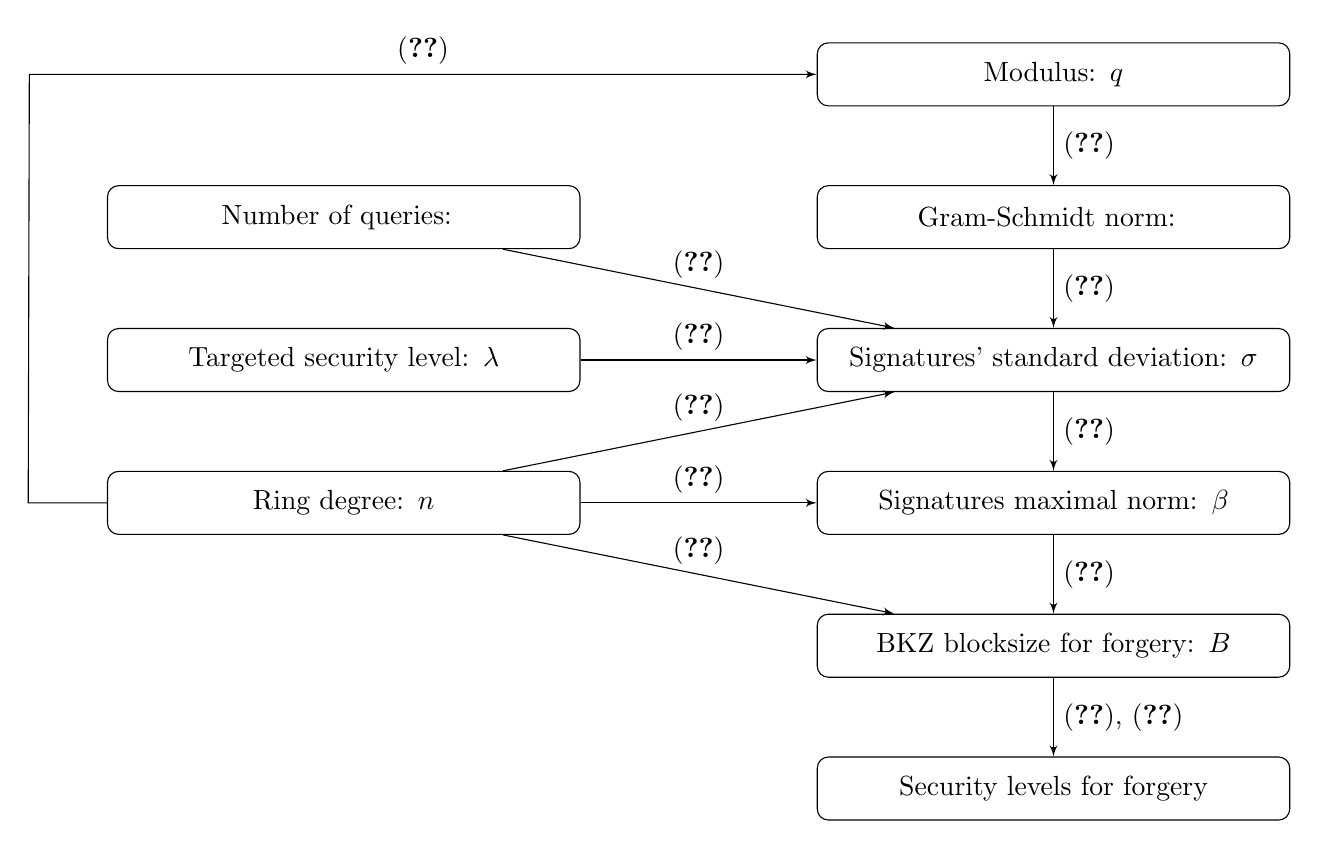
\begin{tikzpicture}[every node/.style={draw=black,anchor=center}, align=center,>={Stealth}]
	\matrix (m) [matrix of nodes,row sep=10mm,column sep = 30mm,draw=none, align=center, text width=60mm, minimum height=8mm, inner sep=0mm, rounded corners]
	{
		& Modulus: $q$ \\
		Number of queries: $\queries$ & Gram-Schmidt norm: $\gsnorm{\matB}$ \\
		Targeted security level: $\lambda$ & Signatures' standard deviation: $\sigma$ \\
		Ring degree: $n$ & Signatures maximal norm: $\beta$ \\
		& BKZ blocksize for forgery: $B$ \\
		& Security levels for forgery \\
	};
	\draw[line] (m-4-1.west) -- ($(m-4-1.west)+(-10mm,0)$) -- ($(m-1-2.west)+(-100mm,0)$) -- node[above,draw=none] {\eqref{eq:q}} (m-1-2.west);
	\draw[line] (m-1-2) -> node[right,draw=none] {\eqref{eq:gsnorm}} (m-2-2);
	\draw[line] (m-2-2) -> node[right,draw=none] {\eqref{eq:sigma:1}} (m-3-2);
	\draw[line] (m-3-2) -> node[right,draw=none] {\eqref{eq:beta}} (m-4-2);
	\draw[line] (m-2-1) -> node[above,draw=none] {\eqref{eq:sigma:1}} (m-3-2);
	\draw[line] (m-3-1) -> node[above,draw=none] {\eqref{eq:sigma:1}} (m-3-2);
	\draw[line] (m-4-1) -> node[above,draw=none] {\eqref{eq:sigma:1}} (m-3-2);
	\draw[line] (m-4-1) -> node[above,draw=none] {\eqref{eq:beta}} (m-4-2);
	\draw[line] (m-4-1) -> node[above,draw=none] {\eqref{eq:blocksize_forgery}} (m-5-2);
	\draw[line] (m-4-2) -> node[right,draw=none] {\eqref{eq:blocksize_forgery}} (m-5-2);
	\draw[line] (m-5-2) -> node[right,draw=none] {\eqref{eq:sec_classic}, \eqref{eq:sec_quantum}} (m-6-2);
	\end{tikzpicture}
	\caption{Parameters of \falcon and security estimates. Initial parameters are on the left side of the figure. Parameters on the right side of the figure (which include concrete security estimates) are derived systematically from initial parameters.}\label{fig:}
\end{figure}

\paragraph{Number of queries $\queries$, targeted security level $\lambda$ and ring degree $n$.} We start with three initial parameters: the maximal number of signing queries $\queries$, the targeted security level $\lambda$ and the degree $n$ of the ring $\bZ[x]/(x^n + 1)$. As per \cite{NIST}, $\queries = 2^{64}$. Also as per \cite{NIST}, it suffices to take $\lambda = 128$ for NIST Level I and $\lambda = 256$ for NIST Level V. Finally, we take:
\begin{align}
& n = 512 && \text{for NIST Level I,}\\
& n = 1024 && \text{for NIST Level V.}
\end{align}

\paragraph{Integer modulus $q$.} The modulus $q$ needs to be a prime of the form $k \cdot 2n + 1$ in order to maximize the efficiency of the NTT. The smallest prime of this form is
\begin{equation}\label{eq:q}
q = 12 \cdot 1024 + 1 = 12289.
\end{equation}
For this value, $q$ has essentially no influence on security: it is large enough to resist hybrid attacks and trivial attacks on SIS, and small enough to resist overstetched NTRU attacks.

\paragraph{Gram-Schmidt norm $\gsnorm{\matB}$.} We wish to minimize $\gsnorm{\matB}$. It has been shown in \cite[Section 3]{AC:DucLyuPre14} that in practice we can ensure (upon resampling a finite number of times) that:
\begin{equation}\label{eq:gsnorm}
\gsnorm{\matB} \leq 1.17 \sqrt{q}.
\end{equation}
In order to do that, each coefficient of $f$ and $g$ is sampled from the discrete Gaussian $D_{\bZ, \sigmafg}$ with:
\begin{equation}\label{eq:sigmafg}
\sigmafg = 1.17 \sqrt{q/2n}.
\end{equation}
%until \eqref{eq:gsnorm} is verified.

\paragraph{Standard deviation $\sigma$ of the signatures.} Signatures are sampled from a discrete Gaussian distribution using the fast Fourier sampling algorithm (with $\matB$ as a basis and a standard deviation $\sigma$). It suffices to take $\epsilon \leq 1 / \sqrt{\queries \cdot \lambda}$ and:
\begin{align}
\sigma & = \frac{1}{\pi} \cdot \sqrt{\frac{\log(4n (1 + 1 / \epsilon))}{2}} \cdot 1.17 \cdot \sqrt{q} \label{eq:sigma:1} \\
& \geq \smooth(\bZ^{2n}) \cdot \gsnorm{\matB} \notag \label{eq:sigma:2}
\end{align}
Following \cite[Lemma 6]{AC:Prest17}, this ensures that $R_{2\lambda}(\cD \cdot \matB \| D_{\Lambda_q^\perp, \sigma, \vecc}) \lesssim 1 + O(1) / \queries$, where $\cD$ is the output of the sampler, $D_{\Lambda_q^\perp, \sigma, \vecc}$ is an ideal Gaussian and $R_{2\lambda}$ is the R\'enyi divergence between them. Following \cite[Section 3.3]{AC:Prest17}, $O(1)$ bits of security are lost by using our sampler instead of $D_{\Lambda_q^\perp, \sigma, \vecc}$.

\paragraph{Maximal norm $\beta$ of the signatures.} During the signing and verification procedures, signatures $(s_1, s_2)$ must verify $\|(s_1, s_2)\|^2 \leq \sqsignorm$ in order to be accepted, with:
\begin{equation}\label{eq:beta}
\beta = \sigrate \cdot \sigma \sqrt{2n}, \hspace*{10mm} \sigrate = \sigrateval
\end{equation}
We call $\sigrate$ the tailcut rate of signatures, because the expected value of $\|(s_1, s_2)\|$ is $\sigma \sqrt{2n}$; any signature larger than this expected value by a factor more than $\sigrate$ is rejected. By applying \cite[Lemma 4.4, Item 3]{EC:Lyubashevsky12}, the probability that a sampled signature is larger than $\beta$ (hence that the signing procedure has to restart) is upper bounded as follows:
\begin{equation}\label{eq:rejrate}
\bP[\|(s_1, s_2)\|^2 > \sqsignorm] \leq \sigrate^{2n} \cdot e^{n \left(1 - \sigrate^{2} \right)}.
\end{equation}
 %TPr: I moved the rationale before the spec
\section{Advantages and Limitations of \falcon}\label{sec:ratio:advantages}

%This section lists the advantages and limitations of \falcon.

\subsection{Advantages}

\paragraph{Compactness.} The main advantage of \falcon is its compactness. This doesn't really come as a surprise as \falcon was designed with compactness as the main criterion. Stateless hash-based signatures often have small public keys, but large signatures. Conversely, some multivariate schemes achieve very small signatures but require large public keys. Lattice-based schemes~\cite{NISTPQC-R2:CRYSTALS-DILITHIUM19} can offer the best of both worlds, but no NIST candidate gets $|\pk|+|\signature|$ to be as small as \falcon does.

\paragraph{Fast signature generation and verification.} The signature generation and verification procedures are very fast. This is especially true for the verification algorithm, but even the signature algorithm can perform more than $1000$ signatures per second on a moderately-powered computer.

\paragraph{Security in the ROM and QROM.} The GPV framework comes with a security proof in the random oracle (ROM), and a security proof in the quantum random oracle model (QROM) was later provided in \cite{AC:BDFLSZ11}. See also \cite{PKC:ChaDeb20}. In contrast, the Fiat-Shamir heuristic has only recently been proven secure in the QROM, and under certain conditions~\cite{C:LiuZha19,C:DFMS19}.

\paragraph{Modular design.} The design of \falcon is modular. Indeed, we instantiate the GPV framework with NTRU lattices, but it would be easy to replace NTRU lattices with another class of lattices if necessary. Similarly, we use fast Fourier sampling as our trapdoor sampler, but it is not necessary either. Actually, an extreme simplicity/speed trade-off would be to replace our fast Fourier sampler with Klein's sampler: signature generation would be two orders of magnitudes slower, but it would be simpler to implement and its black-box security would be the same.

%\paragraph{Message recovery mode.} In some situations, it can be advantageous to use \falcon in message-recovery mode. The signature becomes twice as long but the message does not need to be sent anymore, which induces a gain on the total communication complexity.

\paragraph{Signatures with message recovery.}
In \cite{SCN:delLyuPoi16}, it has been shown that a preliminary version of \falcon can be instantiated in message-recovery mode: the message \msg can be recovered from the signature \signature. It makes the signature twice longer, but allows to entirely recover a message which size is slightly less than half the size of the original signature. In situations where we can apply it, it makes \falcon even more competitive from a compactness viewpoint.

\paragraph{Key recovery mode.} \falcon can also be instantiated in key-recovery mode. In this mode, The signature becomes twice longer but the key is reduced to a single hash value. In addition to incurring a very short key, this reduces the total size $|\pk|+|\signature|$ by about 15\%. More details are given in Section~\ref{sec:key-recovery}.

\paragraph{Identity-based encryption.} As shown in \cite{AC:DucLyuPre14}, \falcon can be converted into an identity-based encryption scheme in a straightforward manner.

\paragraph{Easy signature verification.} The signature procedure is very simple: essentially, one just needs to compute $[H(\salt\|\msg) - s_2 h] \bmod q$, which boils down to a few NTT operations and a hash computation.


\subsection{Limitations}

%\falcon also has a few limitations. These limitations are implementation-related and interestingly, they concern only the signer. We list them below.

\paragraph{Delicate implementation.} We believe that both the key generation procedure and the fast Fourier sampling are non-trivial to understand and delicate to implement, and constitute the main shortcoming of \falcon. On the bright side, the fast Fourier sampling uses subroutines of the fast Fourier transform as well as trees, two objects most implementers are familiar with.

\paragraph{Floating-point arithmetic.} Our signing procedure uses floating-point arithmetic with 53 bits of precision. While this poses no problem for a software implementation, it may prove to be a major limitation when implementation on constrained devices -- in particular those without a floating-point unit -- will be considered.

% \paragraph{Cumbersome key generation.} In \falcon, the key generation is reasonably fast (less than 2 seconds on a moderately-powered computer), but its memory cost is rather high (about $4$ MBytes). Combined to the fact that it requires rather complex operations on multiprecision integers, this fact may preclude the implementation of the key generation procedure on constrained devices.

%\paragraph{Unclear side-channel resistance.} \falcon relies heavily on discrete Gaussian sampling over the integers. How to implement this securely with respect to timing and side-channel attacks has remained largely unstudied, although this has recently started to change~\cite{EPRINT:ZhaSteSak18,DAC:KSVV19,C:MicWal17,EPRINT:RRVV14}.

\medskip

We previously listed ``unclear side-channel resistance'' as a limitation of \falcon, due to discrete Gaussian sampling over the integers. This is much less the case now: constant-time implementations for this step and for the whole scheme are provided in \cite{PQCRYPTO:HPRR20} and \cite{EPRINT:Pornin19}, respectively. A challenging next step is to implement \falcon in a masked fashion.

\input{spec2.tex}
% @author Thomas Prest
% @author Pierre-Alain Fouque
% @author Jeffrey Hoffstein
% @author Paul Kirchner
% @author Vadim Lyubashevsky
% @author Thomas Pornin
% @author Thomas Ricosset
% @author Gregor Seiler
% @author William Whyte
% @author Zhenfei Zhang
% @copyright The authors

\chapter{Implementation and Performances}\label{chap:impl}

We list here a number of noteworthy points related to implementation.

\section{Floating-Point}

Signature generation, and also part of key pair generation, involve the
use of complex numbers. These can be approximated with standard IEEE 754
floating-point numbers (``binary64'' format, commonly known as ``double
precision''). Each such number is encoded over 64 bits, that split into
the following elements:
\begin{itemize}
  \item a sign $s = \pm 1$ (1 bit);
  \item an exponent $e$ in the $-1022$ to $+1023$ range (11 bits);
  \item a mantissa $m$ such that $1\le m< 2$ (52 bits).
\end{itemize}
In general, the represented value is $sm2^e$. The mantissa is encoded as
$2^{52}(m-1)$; it has 53 bits of precision, but its top bit, of value 1
by definition, is omitted in the encoding.

The exponent $e$ uses 11 bits, but its range covers only 2046 values, not
2048. The two extra possible values for that field encode special cases:
\begin{itemize}
  \item The value zero. IEEE 754 has two zeros, that differ by the sign
  bit.
  \item Subnormals: they use the minimum value for the exponent ($-1022$)
  but the implicit top bit of the mantissa is 0 instead of 1.
  \item Infinites (positive and negative).
  \item Erroneous values, known as NaN (Not a Number).
\end{itemize}

Apart from zero, \falcon does not exercise these special cases; exponents
remain relatively close to zero; no infinite or NaN is obtained.

The C language specification does not guarantee that its \verb+double+
type maps to IEEE 754 ``binary64'' type, only that it provides an
exponent range and precision that match at least that IEEE type. Support
of subnormals, infinites and NaNs is left as implementation-defined. In
practice, most C compilers will provide what the underlying hardware
directly implements, and \emph{may} include full IEEE support for the
special cases at the price of some non-negligible overhead, e.g. extra
tests and supplementary code for subnormals, infinites and NaNs. Common
x86 CPU, in 64-bit mode, use SSE2 registers and operations for
floating-point, and the hardware already provides complete IEEE 754
support. Other processor types have only a partial support; e.g. many
PowerPC cores meant for embedded systems do not handle subnormals (such
values are then rounded to zeros). \falcon works properly with such
limited floating-point types.

Some processors do not have a FPU at all. These will need to use
some emulation using integer operations. As explained above, special
cases need not be implemented.

\section{FFT and NTT}

\subsection{FFT}

\todo[inline]{Replace the $\phi, \phi'$ by concrete values}

The Fast Fourier Transform for a polynomial $f$ computes $f(\zeta)$
for all roots $\zeta$ of $\phi$ (over $\bC$). It is normally expressed
recursively. If $\phi = x^n+1$, and $f = f_0(x^2) + xf_1(x^2)$, then
the following holds for any root $\zeta$ of $\phi$:
\begin{equation}
  \begin{array}{rcl}
     f(\zeta) &=& f_0(\zeta^2) + \zeta f_1(\zeta^2) \\
     f(-\zeta) &=& f_0(\zeta^2) - \zeta f_1(\zeta^2)
  \end{array}
\end{equation}
$\zeta^2$ is a root of $x^{n/2}+1$: thus, the FFT of $f$ is easily
computed, with $n/2$ multiplications and $n$ additions or subtractions,
from the FFT of $f_0$ and $f_1$, both being polynomials of degree less
than $n/2$, and taken modulo $\phi' = x^{n/2}+1$. This leads to a
recursive algorithm of cost $O(n \log n)$ operations.

The FFT can be implemented iteratively, with minimal data movement and
no extra buffer: in the equations above, the computed $f(\zeta)$ and
$f(-\zeta)$ will replace $f_0(\zeta^2)$ and $f_1(\zeta^2)$. This leads
to an implementation known as ``bit reversal'', due to the resulting
ordering of the $f(\zeta)$: if $\zeta_j = e^{i(\pi/2n)(2j+1)}$, then
$f(\zeta_j)$ ends up in slot $\text{rev}(j)$, where $\text{rev}$ is the
bit-reversal function over $\log_2 n$ bits (it encodes its input in
binary with left-to-right order, then reinterprets it back as an integer
in right-to-left order).

In the iterative, bit-reversed FFT, the first step is computing the
FFT of $n/2$ sub-polynomials of degree 1, corresponding to source
index pairs $(0,n/2)$, $(1,n/2+1)$, and so on.

Some noteworthy points for FFT implementation in \falcon are the
following:
\begin{itemize}

  \item The FFT uses a table of pre-computed roots $\zeta_j =
  e^{i(\pi/2n)(2j+1)}$. The inverse FFT nominally requires, similarly, a
  table of inverses of these roots. However, $\zeta_j^{-1} =
  \overline{\zeta_j}$; thus, inverses can be efficiently recomputed by
  negating the imaginary part.

  \item $\phi$ has $n$ distinct roots in $\bC$, leading to $n$ values
  $f(\zeta_j)$, each being a complex number, with a real and an
  imaginary part. Storage space requirements are then $2n$
  floating-point numbers. However, if $f$ is real, then, for every root
  $\zeta$ of $\phi$, $\overline\zeta$ is also a root of $\phi$, and
  $\overline{f(\zeta)} = f(\overline\zeta)$. Thus, the FFT
  representation is redundant, and half of the values can be omitted,
  reducing storage space requirements to $n/2$ complex numbers, hence
  $n$ floating-point values.

  \item The Hermitian adjoint of $f$ is obtained in FFT representation
  by simply computing the conjugate of each $f(\zeta)$, i.e. negating
  the imaginary part. This means that when a polynomial is equal to its
  Hermitian adjoint (e.g. $f\adj f+g\adj g$), then its FFT
  representation contains only real values. If then multiplying or
  dividing by such a polynomial, the unnecessary multiplications by $0$
  can be optimized away.

  \item The C language (since 1999) offers direct support for complex
  numbers. However, it may be convenient to keep the real and imaginary
  parts separate, for values in FFT representation. If the real and
  imaginary parts are kept at indexes $k$ and $k+n/2$, respectively,
  then some performance benefits are obtained:
  \begin{itemize}

    \item The first step of FFT becomes free. That step involves
    gathering pairs of coefficients at indexes $(k,k+n/2)$, and
    assembling them with a root of $x^2+1$, which is $i$. The source
    coefficients are still real numbers, thus $(f_0,f_{n/2})$ yields
    $f_0+if_{n/2}$, whose real and imaginary parts must be stored at
    indexes $0$ and $n/2$ respectively, where they already are. The
    whole loop disappears.

    \item When a polynomial is equal to its Hermitian adjoint, all
    its values in FFT representation are real. The imaginary parts
    are all null, and they represent the second half of the array.
    Storage requirements are then halved, without requiring any special
    reordering or move of values.
  \end{itemize}

\end{itemize}


\subsection{NTT}

The \emph{Number Theoretic Transform} is the analog of the FFT, in the
finite field $\bZ_p$ of integers modulo a prime $p$.
$\phi = x^n+1$ will have roots in $\bZ_p$ if and only if $p = 1\bmod
2n$. The NTT, for an input
polynomial $f$ whose coefficients are integers modulo $p$, computes
$f(\omega) \bmod p$ for all roots $\omega$ of $\phi$ in $\bZ_p$.

Signature verification is naturally implemented modulo $q$; that
modulus is chosen precisely to be NTT-friendly:
$$q = 12289 = 1 + 12\cdot 2048.$$
Computations modulo $q$ can be implemented with pure 32-bit integer
arithmetics, avoiding divisions and branches, both being relatively
expensive. For instance, modular addition of \verb+x+ and \verb+y+
may use this function:
\begin{verbatim}
    static inline uint32_t
    mq_add(uint32_t x, uint32_t y, uint32_t q)
    {
        uint32_t d;

        d = x + y - q;
        return d + (q & -(d >> 31));
    }
\end{verbatim}
This code snippet uses the fact that C guarantees operations on
\verb+uint32_t+ to be performed modulo $2^{32}$; since operands fits on
15 bits, the top bit of the intermediate value \verb+d+ will be \verb+1+
if and only if the subtraction of \verb+q+ yields a negative value.

For multiplications, Montgomery multiplication is effective:
\begin{verbatim}
    static inline uint32_t
    mq_montymul(uint32_t x, uint32_t y, uint32_t q, uint32_t q0i)
    {
        uint32_t z, w;

        z = x * y;
        w = ((z * q0i) & 0xFFFF) * q;
        z = ((z + w) >> 16) - q;
        return z + (q & -(z >> 31));
    }
\end{verbatim}
The parameter \verb+q0i+ contains $1/q \bmod 2^{16}$, a value which can
be hardcoded since $q$ is also known at compile-time. Montgomery
multiplication, given $x$ and $y$, computes $xy/(2^{16}) \bmod q$. The
intermediate value \verb+z+ can be shown to be less than $2q$, which is
why a single conditional subtraction is sufficient.

Modular divisions are not needed for signature verification, but they
are handy for computing the public key $h$ from $f$ anf $g$, as part of
key pair generation. Inversion of $x$ modulo $q$ can be computed in
a number of ways; exponentation is straightforward:
$1/x = x^{q-2} \bmod q$. For $12289$, minimal addition
chains on the exponent yield the result in 18 Montgomery multiplications
(assuming input and output are in Montgomery representation).

Key pair generation may also use the NTT, modulo a number of small
primes $p_i$, and the branchless implementation techniques described
above. The choice of the size of such small moduli $p_i$ depends on
the abilities of the current architecture. The \falcon reference
implementation, that aims at portability, uses moduli $p_i$ which
are slightly below $2^{31}$, a choice which has some nice properties:
\begin{itemize}
  \item Modular reductions after additions or subtractions can be
  computed with pure 32-bit unsigned arithmetics.
  \item Values may fit in the \emph{signed} \verb+int32_t+ type.
  \item When doing Montgomery multiplications, intermediate values
  are less than $2^{63}$ and thus can be managed with the standard
  type \verb+uint64_t+.
\end{itemize}
On a 64-bit machine with $64\times 64\rightarrow 128$ multiplications,
63-bit moduli would be a nice choice.

\section{LDL Tree}

From the private key properly said (the $f$, $g$, $F$ and $G$ short
polynomials), signature generation involves two main steps: building the
LDL tree, and then using it to sample a short vector. The LDL tree
depends only on the private key, not the data to be signed, and is
reusable for an arbitrary number of signatures; thus, it can be
considered part of the private key. However, that tree is rather bulky
(about 90~kB for $n = 1024$), and will use floating-point values, making
its serialization complex to define in all generality. Therefore, the
\falcon reference code rebuilds the LDL tree dynamically when the
private key is loaded; its API still allows a built tree to be applied
to many signature generation instances.

It would be possible to regenerate the LDL tree on the go, for a
computational overhead similar to that of sampling the short vector
itself; this would save space, since at no point would the full tree
need to be present in RAM, only a path from the tree root to the current
leaf. For degree $n$, a saved path would amount to about $2n$
floating-point values, i.e. roughly 16~kB. On the other hand,
computational cost per signature would double.

Both LDL tree construction and sampling involve operations on
polynomials, including multiplications (and divisions). It is highly
recommended to use FFT representation, since multiplication and division
of two degree-$n$ polynomials in FFT representation requires only $n$
elementary operations. The LDL tree is thus best kept in FFT.

%\section{Gaussian Sampler}\label{sec:impl:gaussian}
%
%\todo[inline]{Modify to take into account the recent advancements}
%When sampling a short vector, the inner Gaussian sampler is invoked
%twice for each leaf of the LDL tree. Each invocation should produce an
%integer value that follows a Gaussian distribution centered on a value
%$\mu$ and with standard deviation $\sigma$. The centers $\mu$ change
%from call to call, and are dynamically computed based on the message to
%sign, and the values returned by previous calls to the sampler. The
%values of $\sigma$ are the leaves of the LDL tree: they depend on the
%private key, but not on the message; they range between $\sigmin$ and $\sigmax$.
%
%In the \falcon reference code, rejection sampling with regards to a
%bimodal Gaussian is used:
%\begin{itemize}
%
%  \item The target $\mu$ is moved into the $[0..1[$ interval by adding
%  an appropriate integer value, which will be subtracted from the
%  sampling result at the end. For the rest of this description, we
%  assume that $0 \leq \mu < 1$.
%
%  \item A nonnegative integer $z$ is randomly sampled following a half
%  Gaussian distribution of standard deviation $\sigma_0 = 2$, centered
%  on $0$.
%
%  \item A random bit $b$ is obtained, to compute $z' = b + (2b-1)z$.
%  The integer $z'$ follows a bimodal Gaussian distribution, and in
%  the range of possible values for $z'$ (depending on $b$), that
%  distribution is above the target Gaussian of center $\mu$ and
%  standard deviation $\sigma$.
%
%  \item Rejection sampling is applied. $z'$ follows the distribution:
%  \begin{equation}
%    G(z) = e^{-(z-b)^2/(2\sigma_0^2)}
%  \end{equation}
%  and we target the distribution:
%  \begin{equation}
%    S(z) = e^{-(z-\mu)^2/(2\sigma^2)}
%  \end{equation}
%  We thus generate a random bit $d$, whose value is 1 with probability:
%  \begin{equation}\label{eq:rejprob}
%    \begin{array}{rcl}
%      P(d = 1) &=& S(z)/G(z) \\
%      &=& e^{(z-b)^2/(2\sigma_0^2) - (z-\mu)^2/(2\sigma^2)}
%    \end{array}
%  \end{equation}
%  If bit $d$ is $1$, then we return $z'$; otherwise, we start over.
%
%\end{itemize}
%
%Random values are obtained from a custom PRNG; the reference code uses
%ChaCha20, but any PRNG whose output is indistinguishable from random
%bits can be used. On a recent x86 CPU, it would make sense to use AES in
%CTR mode, to leverage the very good performance of the AES opcodes
%implemented by the CPU.
%
%With a careful R\'enyi argument, the 53-bit precision of floating-point values
%used in the sampler computations are sufficient to achieve the required
%security levels.
%
%\tprcomment{Remove/update}
%
%It is worth noting that the Gaussian sampler in the \falcon reference code is
%not constant time, therefore it may be a source of leakage for a side-channel
%attack. Keeping this in mind, since the bimodal Gaussian samples can be drafted
%off-line and the rejection sampling only leaks inaccurate information about the
%secret key (which, based on the state of our knowledge, cannot result in a
%side-channel attack) we did not feel it was necessary to integrate a constant
%time Gaussian sampler in the \falcon reference code. However, we note that
%several proposals~\cite{EPRINT:ZWXZ18,EPRINT:ZhaSteSak18,DAC:KSVV19,
%EPRINT:Walter19} for efficient (constant-time) Gaussian sampling over the
%integers have been made recently and could be used in the bimodal Gaussian
%sampler.
%
%Assuming that the bimodal Gaussian sampler output is unpredictable for an
%attacker (e.g. by using a constant-time algorithm, off-line buffering or
%time-padding techniques), simple adjustments can be made to obtain an execution
%time independant of any secret value:
%\begin{itemize}
%
%  \item The rejection probability is proportional to $\sum_{z=-\infty}^\infty
%  e^{-(z)^2/(2\sigma^2)}$. This sum is actually a theta function and can be
%  approximated by $\sigma\sqrt{2\pi}$. So the probability to return $z'$ is
%  proportional to $\sigma$. However, one can easily remove this dependency by
%  replacing the probability $p := S(z)/G(z)$ in (\ref{eq:rejprob}) by
%  $\frac{\sigma_{\min}}{\sigma} p$. This makes the probability independent of
%  $\sigma$: here, $\sigma_{\min}$ is a lower bound on $\sigma$ (say
%  $\sigma_{\min} = 1.2$) which knowledge is considered not sensitive.
%
%  \item In the \falcon reference code, the $\exp(x)$ implementation is similar
%  to the C standard library which uses a floating-point division. However, the
%  compiler may replace the division operation with its own arithmetic library
%  routine, which may not be constant-time~\cite{EPRINT:Seiler18}. One can
%  easily avoid this division by using a polynomial evaluation at point $x$
%  instead~\cite{EPRINT:ZhaSteSak18}.
%
%\end{itemize}

\section{Key Pair Generation}

\subsection{Gaussian Sampling}

The $f$ and $g$ polynomials must be generated with an appropriate
distribution. It is sufficient to generate each
coefficient independently, with a Gaussian distribution centered on 0;
values are easily tabulated.

\subsection{Filtering}

As per the \falcon specification, once $f$ and $g$ have been generated,
some tests must be applied to determine their appropriateness:
\begin{itemize}

  \item $(g, -f)$ and its orthogonalized version must be short
  enough.

  \item $f$ must be invertible modulo $\phi$ and $q$; this is necessary
  in order to be able to compute the public key $h = g/f \bmod \phi
  \bmod q$. In practice, the NTT is used on $f$: all the resulting
  coefficients of $f$ in NTT representation must be distinct from
  zero. Computing $h$ is then straightforward.

  \item The \falcon reference implementation furthermore requires that
  $\res(f,\phi)$ and $\res(g,\phi)$ be both odd. If they are both even,
  the NTRU equation does not have a solution, but our implementation
  cannot tolerate that one is even and the other is odd. Computing the
  resultant modulo 2 is inexpensive; here, this is equal
  to the sum of the coefficients modulo 2.

\end{itemize}

If any of these tests fails, new $(f,g)$ must be generated.

\subsection{Solving The NTRU Equation}

Solving the NTRU equation is formally a recursive process. At each
depth:
\begin{enumerate}

  \item Input polynomials $f$ and $g$ are received as input; they
  are modulo $\phi = x^n+1$ for a given $n$.

  \item New values $f' = \N(f)$ and $g' = \N(g)$ are computed;
  they live modulo $\phi' = x^{n/2}+1$, i.e. half the degree of $\phi$.
  However, their coefficients are typically twice longer than those of $f$ and $g$.

  \item The solver is invoked recursively over $f'$ and $g'$, and yields
  a solution $(F',G')$ such that $$f'G'-g'F' = q.$$

  \item Unreduced values $(F,G)$ are generated, as:
  \begin{equation}
    \begin{array}{rcl}
      F &=& F'(x^2)g'(x^2)/g(x) \mod \phi \\
      G &=& G'(x^2)f'(x^2)/f(x) \mod \phi
    \end{array}
  \end{equation}
  $F$ and $G$ are modulo $\phi$ (of degree $n$), and their coefficients
  have a size which is about three times that of the coefficients of
  inputs $f$ and $g$.

  \item Babai's nearest plane algorithm is applied, to bring coefficients
  of $F$ and $G$ down to that of the coefficients of $f$ and $g$.

\end{enumerate}

\subsubsection{RNS and NTT}

The operations implied in the recursion are much easier when operating
on the NTT representation of polynomials. Indeed, if working modulo $p$,
and $\omega$ is a root of $x^n+1$ modulo $p$, then:
\begin{equation}
  \begin{array}{rcl}
    f'(\omega^2) &=& N(f)(\omega^2) = f(\omega) f(-\omega) \\
    F(\omega) &=& F'(\omega^2) g(-\omega)
  \end{array}
\end{equation}
Therefore, the NTT representations of $f'$ and $g'$ can be easily computed
from the NTT representations of $f$ and $g$; and, similarly, the NTT
representation of $F$ and $G$ (unreduced) are as easily obtained from
the NTT representations of $F'$ and $G'$.

This naturally leads to the use of a Residue Number System (RNS), in
which a value $x$ is encoded as a sequence of values $x_j = x \bmod p_j$
for a number of distinct small primes $p_j$. In the \falcon reference
implementation, the $p_j$ are chosen such that $p_j < 2^{31}$ (to make
computations easy with pure integer arithmetics) and $p_j = 1 \bmod 2048$
(to allow the NTT to be applied).

Conversion from the RNS encoding to a plain integer in base $2^{31}$ is
a straightforward application of the Chinese Remainder Theorem; if done
prime by prime, then the only required big-integer primitives will be
additions, subtractions, and multiplication by a one-word value. In
general, coefficient values are signed, while the CRT yields values
ranging from $0$ to $\prod p_j - 1$; normalisation is applied by
assuming that the final value is substantially smaller, in absolute
value, than the product of the used primes $p_j$.

\subsubsection{Coefficient Sizes}

Key pair generation has the unique feature that it is allowed occasional
failures: it may reject some cases which are nominally valid, but do not
match some assumptions. This does not induce any weakness or substantial
performance degradation, as long as such rejections are rare enough not
to substantially reduce the space of generated private keys.

In that sense, it is convenient to use \emph{a priori} estimates of
coefficient sizes, to perform the relevant memory allocations and decide
how many small primes $p_j$ are required for the RNS representation of
any integer at any point of the algorithm. The following maximum sizes
of coefficients, in bits, have been measured over thousands of random
key pairs, at various depths of the recursion:

\begin{center}
\begin{tabular}{|c|r|r|r|r|}
\hline
\textbf{\textsf{depth}} & \textbf{\textsf{max} $f$, $g$} & \textbf{\textsf{std. dev.}}
  & \textbf{\textsf{max} $F$, $G$} & \textbf{\textsf{std. dev.}} \\
\hline
 10 & 6307.52 & 24.48 & 6319.66 & 24.51 \\
  9 & 3138.35 & 12.25 & 9403.29 & 27.55 \\
  8 & 1576.87 &  7.49 & 4703.30 & 14.77 \\
  7 &  794.17 &  4.98 & 2361.84 &  9.31 \\
  6 &  400.67 &  3.10 & 1188.68 &  6.04 \\
  5 &  202.22 &  1.87 &  599.81 &  3.87 \\
  4 &  101.62 &  1.02 &  303.49 &  2.38 \\
  3 &   50.37 &  0.53 &  153.65 &  1.39 \\
  2 &   24.07 &  0.25 &   78.20 &  0.73 \\
  1 &   10.99 &  0.08 &   39.82 &  0.41 \\
  0 &    4.00 &  0.00 &   19.61 &  0.49 \\
\hline
\end{tabular}
\end{center}

These sizes are expressed in bits; for each depth, each category of
value, and each key pair, the maximum size of the absolute value is
gathered. The array above lists the observed averages and standard
deviations for these values.

A \falcon key pair generator may thus simply assume that values fit
correspondingly dimensioned buffers, e.g. by using the measured average
added to, say, six times the standard deviation. This would ensure that
values almost always fit. A final test at the end of the process, to
verify that the computed $F$ and $G$ match the NTRU equation, is
sufficient to detect failures.

Note that for depth 10, the maximum size of $F$ and $G$ is the one
resulting from the extended GCD, thus similar to that of $f$ and $g$.

\subsubsection{Binary GCD}

At the deepest recursion level, inputs $f$ and $g$ are plain integers
(the modulus is $\phi = x+1$); a solution can be computed directly with
the Extended Euclidean Algorithm, or a variant thereof. The \falcon
reference implementation uses the binary GCD. This algorithm can be
expressed in the following way:
\begin{itemize}

  \item Values $a$, $b$, $u_0$, $u_1$, $v_0$ and $v_1$ are initialized
  and maintained with the following invariants:
  \begin{equation}
    \begin{array}{rcl}
      a &=& fu_0 - gv_0 \\
      b &=& fu_1 - gv_1
    \end{array}
  \end{equation}
  Initial values are:
  \begin{equation}
    \begin{array}{rcl}
      a &=& f \\
      u_0 &=& 1 \\
      v_0 &=& 0 \\
      b &=& g \\
      u_1 &=& g \\
      v_1 &=& f-1
    \end{array}
  \end{equation}

  \item At each step, $a$ or $b$ is reduced: if $a$ and/or $b$ is even,
  then it is divided by 2; otherwise, if both values are odd, then
  the smaller of the two is subtracted from the larger, and the result,
  now even, is divided by 2. Corresponding operations are applied on
  $u_0$, $v_0$, $u_1$ and $v_1$ to maintain the invariants. Note that
  computations on $u_0$ and $u_1$ are done modulo $g$, while computations
  on $v_0$ and $v_1$ are done modulo $f$.

  \item Algorithm stops when $a = b$, at which point the common value
  is the GCD of $f$ and $g$.

\end{itemize}

If the GCD is 1, then a solution $(F,G) = (qv_0, qu_0)$ can be returned.
Otherwise, the \falcon reference implementation rejects the $(f,g)$
pair. Note that the (rare) case of a GCD equal to $q$ itself is also
rejected; as noted above, this does not induce any particular algorithm
weakness.

The description above is a bit-by-bit algorithm. However, it can be seen
that most of the decisions are taken only on the low bits and high bits
of $a$ and $b$. It is thus possible to group updates of $a$, $b$ and
other values by groups of, say, 31 bits, yielding much better
performance.

\subsubsection{Iterative Version}

Each recursion depth involves receiving $(f,g)$ from the upper level,
and saving them for the duration of the recursive call. Since degrees
are halved and coefficients double in size at each level, the storage
space for such an $(f,g)$ pair is mostly constant, around 13000 bits per
depth. For $n = 1024$, depth goes to 10, inducing a space requirement of
at least 130000 bits, or 16~kB, just for that storage. In order to
reduce space requirements, the \falcon reference implementation
recomputes $(f,g)$ dynamically from start when needed. Measures
indicate a relatively low CPU overhead (about 15\%).

A side-effect of this recomputation is that each recursion level
has nothing to save. The algorithm thus becomes iterative.

\subsubsection{Babai's Reduction}

When candidates $F$ and $G$ have been assembled, they must be reduced
against the current $f$ and $g$. Reduction is performed as successive
approximate reductions, that are computed with the FFT:
\begin{itemize}

  \item Coefficients of $f$, $g$, $F$ and $G$ are converted to
  floating-point values, yielding $\dot f$, $\dot g$, $\dot F$ and $\dot
  G$. Scaling is applied so that the maximum coefficient of $\dot F$ and
  $\dot G$ is about $2^{30}$ times the maximum coefficient of $\dot f$
  and $\dot g$; scaling also ensures that all values fit in the exponent
  range of floating-point values.

  \item An integer polynomial $k$ is computed as:
  \begin{equation}
    k = \left\lfloor \frac{\dot F\dot f^\star + \dot G\dot g^\star}{\dot f\dot f^\star + \dot g\dot g^\star} \right\rceil
  \end{equation}
  This computation is typically performed in FFT representation, where
  multiplication and division of polynomials are easy. Rounding to
  integers, though, must be done in coefficient representation.

  \item $kf$ and $kg$ are subtracted from $F$ and $G$, respectively.
  Note that this operation must be exact, and is performed on the
  integer values, not the floating-point approximations. At high degree
  (i.e. low recursion depth), RNS and NTT are used: the more efficient
  multiplications in NTT offset the extra cost for converting values to
  RNS and back.

\end{itemize}

This process reduces the maximum sizes of coefficients of $F$ and $G$ by
about 30 bits at each iteration; it is applied repeatedly as long as it
works, i.e. the maximum size is indeed reduced. A failure is reported if
the final maximum size of $F$ and $G$ coefficients does not fit the
target size, i.e. the size of the buffers allocated for these values.

%\newpage

\section{Performances}\label{sec:impl:perf}

The \falcon reference implementation achieves the following performance
on an Intel® Core® i5-8259U CPU (``Coffee Lake'' core, clocked at
2.3~GHz):

\begin{center}
\begin{tabular}{|c|r|r|r|r|r|r|}
\hline
\textbf{\textsf{degree}} & \textbf{\textsf{keygen (ms)}}
  & \textbf{\textsf{keygen (RAM)}} & \textbf{\textsf{sign/s}}
  & \textbf{\textsf{vrfy/s}} & \textbf{\textsf{pub length}}
  & \textbf{\textsf{sig length}} \\
\hline
512  &  8.64 & 14336 & 5948.1 & 27933.0 &  897 &  \sigbytelenvali \\
%768  & 12.69 & 27648 & 3547.9 & 20637.7 & 1441 &  993.91 \\
1024 & 27.45 & 28672 & 2913.0 & 13650.0 & 1793 &  \sigbytelenvalv \\
\hline
\end{tabular}
\end{center}

The following notes apply:
\begin{itemize}

  \item For this test, in order to obtain stable benchmarks, CPU
  frequency scaling (``TurboBoost'') has been disabled. This CPU can
  nominally scale its frequency up to 3.9~GHz (for short durations), for
  a corresponding increase in performance. In particular, since all
  operations at degree 512 fit in L1 cache (both code and data), one may
  expect performance to be proportional to frequency, up to about 10000
  signatures per second at the maximum frequency. The figures shown
  above are for \emph{sustained} workloads in which signatures are
  repeatedly computed over prolonged periods of time.

  \item RAM usage for key pair generation is expressed in bytes. It
  includes temporary buffers for all intermediate values, including
  the floating-point polynomials used for Babai's reduction.

  \item Public key length and average signature length are expressed in
  bytes. The size of public keys includes a one-byte header that
  identifies the degree and modulus. For signatures, compression and
  padding is used, thus leading to a fixed signature length.

  \item Signature generation time does not include the LDL tree
  building, which is done when the private key is loaded. These figures
  thus correspond to batch usage, when many values must be signed with a
  given key. This matches, for instance, the use case of a busy TLS
  server. If, in a specific scenario, keys are used only once, then the
  LDL tree building cost must be added to each signature attempt; this
  almost doubles the signature cost, but reduces RAM usage.

  \item The implementation used for this benchmark is fully constant-time.
  It uses AVX2 and FMA opcodes for improved performance. Compiler is
  Clang 10.0, with optimization flags:\\ \verb+-O3 -march=skylake+.

\end{itemize}


% \chapter{Fast Fourier sampling for dummies}\label{chap:ffs}


\section{Introduction}

\subsection{Roadmap}

\section{Preliminaries}\label{sec:ffs:prelim}

% \subsection{Rings and matrices over Rings}
%
% Let $\phi \in \bR[x]$ be a monic polynomial with distinct roots over $\bC$, $\cR = \bR[x]/(\phi(x))$ be a polynomial quotient ring and $a,b$ be arbitrary elements of $\cR$.
% \begin{itemize}
%  \item
%  We note $\adj{a}$ and call (Hermitian) adjoint of $a$ the unique element of $\cR$ such that for any root $\zeta$ of $\phi$, $\adj{a}(\zeta) = \overline{a(\zeta)}$, where $\overline{\cdot}$ is the usual complex conjugation over $\bC$. We can extend this definition to matrices: the adjoint of a matrix $\matB \in \cR^{n\times m}$ is the coefficient-wise adjoint of the transpose of $\matB$.
%  \item
%  The inner product over $\cR$ is $ \inner{a}{b} = \frac{1}{\deg(\phi)}\sum_{\phi(\zeta)=0} a(\zeta)\cdot \overline{b(\zeta)} = \frac{1}{\deg(\phi)} \fft(a) \cdot \adj{\fft(b)}$, and the associated norm is $\|a\| = \sqrt{\inner{a}{a}}$. This definition extends to vectors $\veca,\vecb$ of $\cR^m$: $\inner{\veca}{\vecb} = \sum_i \inner{a_i}{b_i}$.
% \end{itemize}
% The reason of the presence of the scaling factor $\frac{1}{\deg(\phi)}$ in the definition of the inner product is to make it coincide with the usual coefficient dot product $\inner{a}{b}_2 = \sum_i a_i b_i$ in useful cases: when $\phi(x) = x^n \pm 1$, $\inner{a}{b} = \inner{a}{b}_2 $ for any $a,b \in \bR[x]/(\phi(x))$. However, we note that in general the inner product $\inner{\cdot}{\cdot}$ and the coefficient dot product $\inner{\cdot}{\cdot}_2$ (resp. the norm $\|\cdot\|$
% and the coefficient norm $\|\cdot\|_2$) do not coincide. This difference is not inocuous, and in \falcon{} we systematically use the inner product $\inner{\cdot}{\cdot}$ and its associated norm $\|\cdot\|$, unless stated otherwise.

\paragraph{Linearization operators: a first attempt.} For a polynomial ring $\cR = \bR[x]/(\phi(x))$ of extension degree $d=\deg(\phi)$ over $\bR$, it is often convenient to represent vectors of $\cR^m$ (resp. matrices of $\cR^{m\times n}$) as vectors of $\bR^{md}$ (resp. matrices of $\bR^{md\times nd}$). We lose the ring structure, but in exchange some useful operations (such as orthogonalization) can be done at a fainer-grained level. For vectors of $\cR^m$, this can be done simply by applying the \fft{} component-wise -- which we note $\fft(\vecv)$. For matrices, we define the linear map $\cC : \cR^{n\times m} \rightarrow \bC^{dn \times dm}$ as follows. First, for any $a\in \cR$, the circulant matrix of $a$ is

 \begin{equation}
\cC(a) = \begin{bmatrix*}[c]   \fft(a) \\
\fft(xa) \\
 \vdots \\
\fft(x^{d-1}a) \\ \end{bmatrix*} \in \bC^{d\times d}.
\end{equation}
This definition generalizes to matrices by component-wise application. One can check that for any vector $\vecv$ and matrices $\matB,\matC$ such that the products $\vecv \matB$ and $\matB \matC$ are defined, the map $\cC$ satisfy the following properties:
\begin{enumerate}
 \item
 $\cC$ is an injective algebra morphism. In particular, $\cC(\matB) \cC(\matC) = \cC(\matB \matC)$.
 \item\label{item:circ}
 $\fft(\vecv)\cC(\matB) = \fft(\vecv \matB)$.
\end{enumerate}

The second point illustrates that the maps $\fft$ and $\cC$ are complementary. Indeed, for $a\in \cR$, the $\fft$ maps $a$ to its unique decomposition according to a basis $(e_1,\dots,e_{\deg(\phi)})$. For the same basis, $\cC(a)$ is the transformation matrix of the injective map $f \in \cR \mapsto f a$. This is the intrinsic reason that makes these two properties valid. In addition, $\cC$ allows to easily compute the inner product of elements $x^i a, x^j b\in\cR$: indeed, $\cC(a) \times \adj{\cC(b)} = (\inner{x^i a}{x^j b})_{i,j}$

One can intuitively see why the map $\fft$ and $\cC$ may not be optimal: they interpret $\cR$ (resp. the algebra $\text{End}(\cR)$ of endomorphisms of $\cR$) as a $\bR$-module of dimension $\deg(d)$, without accounting for potential additional structure, like the fact that $\cR$ may belong to a tower of rings. In section~\ref{sec:ffs:prelim:klein}, we will show that this is a limitation of the maps $\fft$ and $\cC$ when using Klein's sampler. In Section~\ref{sec:ffs:prelim:cyclo}, we will define maps $\Ve,\Ma$ analogous to $\fft,\cC$ but which truly exploit tower of rings structures.



\subsection{Gram-Schmidt orthogonalization and the LDL decomposition}\label{sec:ffs:prelim:gso}

% \paragraph{Full-rank matrices.}
% Let $\matB \in \cR^{n \times m}$. We say that $\matB$ is full-rank (or is a basis) if for any linear combination $ \sum a_i \vecb_i$ with $a_i \in \cR$, we have the equivalence $(\sum_i a_i \vecb_i = \veczero) \Longleftrightarrow (\forall i, a_i = 0)$.
%
% We note that since $\cR$ is generally not an integral domain, a set formed of a single nonzero vector is not necessarily full-rank. In the rest of the paper, a basis will either denote a set of independent vectors $\{\vecb_1,\ldots\vecb_n\} \in (\cR^m)^n$, or the full-rank matrix $\matB \in \cR^{n \times m}$ whose rows are the $\vecb_i$'s.
%
% We say that a self-adjoint matrix $\matG \in \cR^{n \times n}$ is full-rank Gram if there exist $m \geq n$ and a full-rank matrix $\matB \in \cR^{n \times m}$ such that $\matG = \matB \adj\matB$. This generalizes the notion of positive definiteness for symmetric real matrices.

\paragraph{The Gram-Schmidt orthogonalization.}
Any matrix $\matB \in \cR^{n \times m}$ can be decomposed as follows:
\begin{equation}
 \matB = \matL \times \tBB,
\end{equation}
where $\matL$ is lower triangular with only $1$'s on the diagonal, and the rows $\tBB$ are pairwise orthogonal. When $\matB$ is full-rank , this decomposition is unique, and it is called the Gram-Schmidt orthogonalization.
We will also call Gram-Schmidt norm of $\matB$ the following value:
\begin{equation}
 \gsnorm{\matB} = \max_{\tilde\vecb_i \in \tBB} \|\tilde\vecb_i\|.
\end{equation}

\paragraph{The $\LDLs$ decomposition.} Closely related to the Gram-Schmidt orthogonalization is the Gram-Shmidt decomposition. The $\LDLs$ decomposition writes any full-rank Gram matrix as a product $\L \matD \adj\L$, where $\matL \in \cR^{n\times n}$ is lower triangular with $1$'s on the diagonal, and $\matD \in \cR^{n\times n}$ is diagonal. It can be computed using algorithm~\ref{alg:ldl}.

%  \begin{algorithm}
%  \caption{$\ldlalgo(\matG)$}\label{alg:ldl}
%  \begin{algorithmic}[1]
%  \Require {A full-rank Gram matrix $\matG = (G_{ij}) \in \cR^{n\times n}$.}
%  \Ensure {The decomposition $\matG = \L \matD \adj\L$ over $\cR$, where $\L$ is unit lower triangular and $\matD$ is diagonal.}
%  \State{$\L, \matD \gets \matzero^{\ n\times n}$}
%  \For{$i$ from $1$ to $n$}
%  \State{$\l_{ii} \gets 1$}
%  \State {$D_{i} \gets G_{ii} - \sum_{j<i} \l_{ij} \adj \l_{ij} D_j$}
%  \For{$j$ from $1$ to $i-1$}
%  \State {$\l_{ij} \gets \frac{1}{D_{j}} \left( G_{ij} -  \sum_{k<j} \l_{ik} \adj \l_{jk} D_k \right)$}
%  \EndFor
%  \EndFor
%  \Return{$((\l_{ij}),\Diag_i(D_i))$}
%  \end{algorithmic}
%  \end{algorithm}

 The $\LDLs$ decomposition and the \gso{} are closely related as for a basis $\matB$, there exists a unique \gso{} $\matB = \L \cdot \tBB$ and for an FRG matrix $\matG$, there exists a unique $\LDLs$ decomposition $\matG = \L  \matD  \adj\L$. If $\matG = \matB \adj \matB$, then $\matG = \L \cdot (\tBB \adj \tBB) \cdot \adj\L$ is a valid $\LDLs$ decomposition of $\matG$. As both decompositions are unique, the matrices $\L$ in both cases are actually the same. In a nutshell:
\begin{equation}
 \left[\L\cdot\tBB \text{ is the \gso{} of } \matB \right]
  \Leftrightarrow  \left[ \L \cdot (\tBB\adj \tBB) \cdot \adj\L  \text{ is the $\LDLs$ decomposition of }(\matB\adj \matB)\right].
\end{equation}
The reason why we present both equivalent decompositions is because the \gso{} allows to provide a more intuitive explanation of Klein's sampler, whereas the use of $\LDLs$ decomposition is faster and therefore makes more sense from an algorithmic point of view.

\subsection{Klein's sampler}\label{sec:ffs:prelim:klein}


Klein's sampler is historically the first trapdoor sampler. Its existence actually predates the very concept of trapdoor sampling, since it was first used in a different context~\cite{SODA:Klein00}. It is defined for lattices over $\bR^m$ and is described in algorithm~\ref{alg:klein}.

 \begin{algorithm}[H]
 \caption{$\klein(\vect, \L, \matD, \sigma)$}
 \label{alg:klein}
 \begin{algorithmic}[1]
 \Require { The $\LDLt$ decomposition $\matB \matB^\t  = \L \cdot \matD \cdot \L^\t$ for $\matB\in \bR^{n\times m}$, a vector $\vect \in \bR^n$}
 \Ensure { A vector $\vecz \in \bZ^n$ such that $\vecz \cdot \matB \sim D_{\Lambda(\matB), \sigma, \vect \matB}$}
 \For{$j = n,\ldots,1$}
 \State{$\bar{t}_j \gets  t_j + \sum_{i>j} (t_i - z_i) \l_{ij}$}
 \State{$\sigma_j \gets \sigma/\sqrt{D_{jj}}$}
 \State{$z_j \gets \gaussround{\bar{t}_j}{\sigma_i}$}
 \EndFor
 \Return{$\vecz$}
  \end{algorithmic}
 \end{algorithm}
 Klein's sampler is a randomized version of the nearest plane algorithm~\cite{STACS:Babai85,Combinatorica:Babai86}. The latter is deterministic and outputs vectors in $[-1,1]^m \cdot \matB$. In Klein's sampler, the rounding at each step $j$ is replaced by a discretized Gaussian of parameter $\sigma_j = \sigma/\|\tilde\vecb_j\|$. It has been shown that if $\sigma \geq \smooth(\bZ^m) \cdot \gsnorm{\matB}$ for a suitable $\epsilon$, then $\klein(\vect, \L, \matD, \sigma) \cdot \matB$ is statistically close to the ideal Gaussian oracle $D_{\Lambda(\matB), \sigma, \vect \matB}$ under various metrics of closeness: the statistical distance~\cite{AC:DucNgu12a}, the Kullback-Leibler divergence~\cite{AC:DucLyuPre14} or the R\'enyi divergence~\cite{AC:Prest17}. This is illustrated by the figure~\ref{fig:nptoklein}.


 \begin{figure}[H]
 \centering
$\begin{array}{ccc}
 \fbox{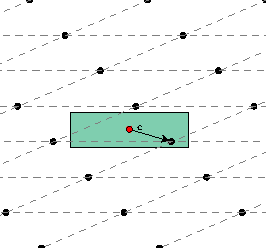
\includegraphics{tikz/BabaiNP}}  &\Longrightarrow& \fbox{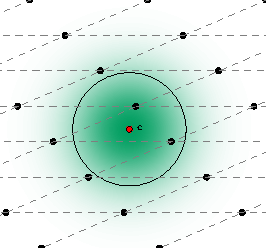
\includegraphics{tikz/Klein}} \\
 \text{Nearest plane algorithm} & & \text{Klein's sampler} \\
\end{array}$
\caption{From the nearest plane algorithm to Klein's sampler.}\label{fig:nptoklein}
\end{figure}


Klein's sampler works only with matrices having coefficients in $\bR$. If we are to work in a ring $\cR = \bR[x]/(x^d\pm 1)$ instead, a straightforward approach to use it while preserving its good security properties is to interpret $\cR$ as a $\bR$-module of dimension $d$. This is done by replacing the vector $\vect \in \cR^{n}$ with $c(\vect)$, and the matrices $\matB, \matB \adj\matB$ with the block circulant matrices $\cC(\matB), \cC(\matB \adj\matB)$.

The problem with this approach is that this interpretation of $\cR$ as a $\bR$-module completely breaks the ring structure that $\cR$ enjoys. As a consequence, the $\LDLs$ decomposition has no obvious structure that Klein's sampler could exploit: its total complexity becomes $O(n^2d^2)$.


% \subsection{Cyclotomic rings}\label{sec:ffs:prelim:cyclo}
% This section gives a few reminders about cyclotomic polynomials and rings, especially for the rings of interests in the \falcon{} scheme. For $d \in \bN^\star$, $\zeta_d$ denotes an arbitrary primitive $d$-th root of unity in $\bC$, for example $\zeta_d = e^{\frac{2i\pi}{d}}$. We may note $\Omega_d = \{\zeta_d^k | k \in\bZ_d^\times \}$ the set of primitive $d$-th roots of unity. Let
% \begin{equation}
% \phi_d(x) = \prod\limits_{\zeta \in \Omega_d} (x - \zeta) = \prod\limits_{k\in\bZ_d^\times} (x - \zeta_d^k).
% \end{equation}
%
% This polynomial is in $\bZ[x]$ and is called the $d$-th cyclotomic polynomial.
% It is immediate that for any $d$, the degree of $\phi_d$ is $\varphi(d)$, where $\varphi(d) = |\bZ_d^\times|$ is Euler's totient function. For special values of $d$, the cyclotomic polynomial $\phi_d$ is easy to compute:
% \begin{itemize}
%  \item If $d=2^k$ for $k \geq 1$, then $\phi_d(x) = \phi_2(x^{d/2}) = x^{d/2}+1$.
% %  \item If $d=2^k \cdot 3^\ell$ for $k \geq 1$ and $\ell \geq 2$, then $\phi_d = \phi_{18}(x^{d/18}) = x^{d/3} - x^{d/6} + 1$.
% \end{itemize}
% We will also note $\cR_d = \bR[x]/(\phi_d)$ and $\cZ_d = \bZ[x]/(\phi_d)$.
%
% \paragraph{Switching between representations.} For any cyclotomic ring $\bR[x]/(\phi_d)$ and any element $f = \sum_{i=0}^{\phi(d)-1} f_i x^i \in \bR[x]/(\phi_d)$, one may easily switch between the representation $\vecf = (f_i)_{0\leq i< \varphi(d)}$ of $f$ in the coefficient embedding and its representation $\hat\vecf = (f(\zeta))_{\{\phi_d(\zeta)=0\}}$ in the canonical embedding via the fast Fourier transform which, when $d$ is highly composite, can be computed in time $O(d \log d)$.
%
% Another noteworthy property is that for the cases which interest us, computing $\inner{f}{g}$ from $\vecf,\vecg$ and $\inner{f}{g}_2$ from $\hat\vecf,\hat\vecg$ can be done in time $O(d)$ without having to perform any (inverse) fast Fourier transform.
% Indeed, $\hat\vecf = \vecf\cdot \matV_d$, where $\matV_d$ is a Vandermonde matrix: $\matV_d = (\zeta_d^{ij})_{\{0 \leq i < \phi(d), j \in \bZ_d^\times\}}$. Therefore:
% \begin{itemize}
%  \item $\inner{f}{g} = \frac{1}{\phi(d)} \hat\vecf \cdot \hat\vecg^\star = \frac{1}{\phi(d)} \vecf \cdot \matV \times \adj{\matV} \cdot \adj\vecg$.
%  \item $\inner{f}{g}_2 = \vecf \cdot \vecg^\t = \hat\vecf \cdot (\matV \times \adj{\matV})^{-1} \cdot \hat\vecg^{-\star}$.
% \end{itemize}
% For the values of $d$ used in \falcon{}, $\matV_d \times \adj\matV_d $ can be expressed simply:
% \begin{itemize}
%  \item If $d=2^k$ for $k \geq 1$, then $\matV_d \times \adj\matV_d = \phi(d) \matI_{\phi(d)}$.
%  \item If $d=2^k \cdot 3^\ell$ for $k \geq 1$ and $\ell \geq 2$, then we have $\matV_d \times \adj\matV_d = \phi(d) \left[ \matI_{\phi(d)} + \frac{1}{2} \matJ_{\phi(d)}\right]$ and $(\matV_d \times \adj\matV_d )^{-1} = \frac{4}{3\phi(d)} \left[ \matI_{\phi(d)} - \frac{1}{2} \matJ_{\phi(d)}\right]$, for $\matJ_n = \twotwo{\matzero_{n/2}}{\matI_{n/2}}{\matI_{n/2}}{\matzero_{n/2}}$.
% \end{itemize}
%
%
% These are the only properties which are needed in \falcon{}. For additional documentation about cyclotomic polynomials, rings and fields, the readers can refer to e.g.~\cite{Lang95}, Chapter IV.
%
% % \subsection{Linearization operators}\label{sec:ffs:prelim:lin}
%
% TODO:
% \begin{itemize}
%  \item Interpretation: $\Ve$ is a natural way of breaking down the ring $\cR_d$ into a product of smaller rings. It is an isomorphism, so for $\Ve: \cR_d \rightarrow \cR_{d'}^k$ we have that $\cR_{d'}^k$ is itself a ring with the operations induced by this isomorphism: for $\vecx, \vecy \in \cR_{d'}^k$, $\vecx \vecy = \Ve( \Ve^{-1}(\vecx) \Ve^{-1}(\vecy) )$.
%  \item + example for power of two cyclotomics
%  \item $\Ma$ writes the transformation matrix of the map $f \mapsto fa$
% \end{itemize}
%
% \paragraph{Tower of rings.} A convenient fact about cyclotomic polynomials is that they can often be envisioned as parts of tower of rings. We make the following observation:
% \begin{itemize}
% \item
% Any cyclotomic ring $\bR[x]/(\phi_{2d}(x))$ lives as a subring of  $\bR[y]/(\phi_{4d}(y))$ via the morphism $x \mapsto y^2$
% % \item
% % Any cyclotomic ring $\cR = \bR[x]/(\phi(x))$ -- in particular $\bR[x]/(\phi_{18}(x))$ -- can be viewed as a $\bR$-linear space of dimension $\deg(\phi)$ via the morphism $f \in \cR \mapsto \fft(f) \in \bC^{\deg(\phi)}$.
% \end{itemize}
%
% From this, it follows that the base rings used in \falcon{} sit atop tower of rings as decribed below:
% \begin{itemize}
% \item
% For $\lambda = 128$: $\bR = \cR_2 \subsetneq \cR_4 \subsetneq \cR_8 \subsetneq \cR_{16} \subsetneq \cR_{32} \subsetneq \cR_{64} \subsetneq \cR_{128} \subsetneq \cR_{256} \subsetneq \cR_{512}$.
% % \item
% % For $\lambda = 192$: $\bR = \cR_2 \subsetneq \cR_{18} \subsetneq \cR_{36} \subsetneq \cR_{72} \subsetneq \cR_{144} \subsetneq \cR_{288} \subsetneq \cR_{576} \subsetneq \cR_{1152} \subsetneq \cR_{2304}$.
% \item
% For $\lambda = 256$: $\bR = \cR_2 \subsetneq \cR_4 \subsetneq \cR_8 \subsetneq \cR_{16} \subsetneq \cR_{32} \subsetneq \cR_{64} \subsetneq \cR_{128} \subsetneq \cR_{256} \subsetneq \cR_{512} \subsetneq \cR_{1024}$.
% \end{itemize}
%
% Now, the next step is to devise linearization operators similar to the $\fft$ and $\cC$. Unlike the $\fft$ (resp. $\cC$) which directly maps $\cR = \bR[x]/(\phi(x))$ (resp. $\text{End}(\cR)$) to $\bC^{\deg\phi}$, these maps procede in a more gradual way by allowing to decompose $\cR$ over intermediate rings $\cR'$ such that $\bR \subsetneq \cR' \subsetneq \cR$.
%
% \paragraph{The linearization operators $\Ve$ and $\Ma$.}
% Let $d,d'\in \bN^\star$ such that $d'$ divides $d$ strictly (noted $d'|d$). We define the ring-splitting maps $\V{d}{d'}:\cR_d^m \rightarrow \cR_{d'}^{md/d'}$ and $\M{d}{d'} : \cR_d^{n\times m} \rightarrow \cR_{d'}^{(nd/d') \times (md/d')}$ by induction as follows:
% \begin{itemize}
% \item
% If $d$ is a multiple of $4$ and $d'=d/2$, let $a$ be an arbitrary element of $\cR_d$. $a$ can be uniquely decomposed as $a(x) = a_0(x^2) + x a_1(x^2)$, with $a_0, a_1 \in \cR_{d'}$. We then define $\V{d}{d'}(a) = (a_0,a_1)$ and
% \begin{equation}
% \M{d}{d'}(a) = \twotwo{a_0}{a_1}{y a_1}{a_0} = \twoone{\V{d}{d'}(a)}{\V{d}{d'}(xa)}.
% \end{equation}
% % \item
% % If $d$ is a multiple of $2$ but not of $4$ and $d'=2$, then we fall back to the ``classical'' maps $\fft,\cC$: $\V{d}{d'}(a) = \fft(a)$ and $\M{d}{d'}(a) = \cC(a)$.
% \item
% We extend the definition of $\V{d}{d'}$ (resp. $\M{d}{d'}$) to vectors (resp. matrices) by component-wise application.
% \item
% For $d''|d'|d$, we define $\V{d}{d''}$ and $\M{d'}{d''}$ by induction:
% \begin{equation}
%  \V{d}{d''} = \V{d'}{d''} \circ \V{d}{d'} \text{ and } \M{d}{d''} = \M{d'}{d''} \circ \M{d}{d'}.
% \end{equation}
%
% \end{itemize}
% When clear from context, we may omit $d,d'$ in the notations as explained hereinafter. For $\vecv \in \cR_{d}^m$ and $\matB \in \cR_{d}^{n\times m}$, we note $\Ve(\vecv) = \V{d}{(d/2)}(\vecv)$ (resp. $\Ma(\matB) = \M{d}{(d/2)}(\matB)$).
% % , where $d'$ is the largest value for which $\V{d}{d'}(\vecv)$ (resp. $\M{d}{d'}(\matB)$) is defined (which is either $d/2$ or $2$).
% In our algorithms, we will use $\Ve$ and $\Ma$ as often as possible, as they allow to ``gently'' descent down tower of rings.
%
%
% \section{Preprocessing the basis: Fast Fourier orthogonalization}\label{sec:ffs:ffo}
%
% Our goal is now to use the linearization operators $\Ve,\Ma$
%
%  \begin{algorithm}[H]
%  \caption{$\ffldl(\matG)$}\label{alg:ffldl}
%  \begin{algorithmic}[1]
%  \Require {A full-rank Gram matrix $\matG \in \cR_{d}^{n\times n}$}
%  \Ensure {\small The compact $\LDLt$ decomposition of $\matG$ in FFT form}
%  \State {$(\L,\matD) \leftarrow \ldlalgo(\matG)$}\label{step:ldl}
%   \If{$d=2$}
%  \Return{$(\L,\matD)$}
%  \EndIf
%  \For{$i=1,\ldots,n$}
%  \State {$\tL_i \leftarrow \ffldl(\Ma(\matD_{ii}))$}\label{step:ffldl}
%  \EndFor
%  \Return $(\L, (\tL_i)_{1\leq i\leq n})$
%  \end{algorithmic}
%  \end{algorithm}
%
% \section{Trapdoor sampling: the Fast Fourier sampler}\label{sec:ffs:ffs}
%
%
% % TODO:
% % \begin{itemize}
% %  \item Many, many things
% %  \item handle precision issues
% %  \item R\'enyi argument
% % \end{itemize}
%
%  \begin{algorithm}[H]
%   \caption{$\ffklein_{\cR_d}(\vect, \tL, \sigma)$}\label{alg:ffnp}
%  \begin{algorithmic}[1]
%   \Require {$\vect \in \cR_d^n$, a precomputed tree $\tL$, (implicitly) a matrix $\matB \in \cR_d^{n \times m}$ such that $\tL$ is the compact $\LDLt$ decomposition tree of $\matB\adj \matB$.}
%   \Ensure {$\vecz \in \cZ_d^n$ such that $\vecz \cdot \matB \sim D_{\Lambda(\matB), \sigma, \vect \matB}$.}
%   \If{$d=2$}\label{step:bottom1}
%   \State $(\matL, \matD) \gets \tL $
%   \Return{$\klein(\vect, \L, \matD, \sigma)$}\label{step:bottom2}
%   \EndIf\label{step:bottom3}
%  \State{$(\L, (\tL_i)_{1\leq j\leq n}) \leftarrow \tL$}
%  \For{$j = n,\ldots,1$}
%  \State{$\btt_j \leftarrow  \vect_j + \sum_{i>j} (\vect_i - \vecz_i) \l_{ij}$}\label{step:np}
%  \State{$\vecz_j \leftarrow \Ve^{-1} \left[\ffklein( \Ve(\btt_j), \tL_j, \sigma) \right]$}\label{step:ffnp}
%  \EndFor
%  \Return{$ \vecz = (\vecz_i,\dots,\vecz_n)$}
%   \end{algorithmic}
%  \end{algorithm}
%
%  \paragraph{Indistinguishability from an ideal Gaussian.} If $\sigma \geq \smooth(\bZ) \cdot \gsnorm{\matB}$, then the ratio between the distribution $\ffklein_{\cR_d}(\vect, \tL, \sigma) \cdot \matB$ and the ideal Gaussian is always between $\left(\frac{1-\epsilon}{1+\epsilon}\right)^{n \varphi(d)}$ and $\left(\frac{1-\epsilon}{1+\epsilon}\right)^{n \varphi(d)}$. This can be shown by applying inductively the original proof from~\cite{STOC:GenPeiVai08}. The relative error between the two is therefore bounded by approximately $2n \varphi(d) \epsilon $. Following the security arguments from \cite[Section 3.3]{AC:Prest17}, as long as:
%  \begin{equation}
%  \epsilon \leq \frac{1}{n \varphi(d) \sqrt{\lambda q_s}},
%  \end{equation}
% we can replace the ideal Gaussian with the fast Fourier sampler and it will make \falcon{} lose at most one bit of security.
\appendix
% % @author Thomas Prest
% @author Pierre-Alain Fouque
% @author Jeffrey Hoffstein
% @author Paul Kirchner
% @author Vadim Lyubashevsky
% @author Thomas Pornin
% @author Thomas Ricosset
% @author Gregor Seiler
% @author William Whyte
% @author Zhenfei Zhang
% @copyright The authors

\chapter{Gaussian Sampling}


{\small
\bibliography{bib/abbrev2,bib/crypto_crossref,bib/other_biblio}}


\end{document}
